
% Default to the notebook output style

    


% Inherit from the specified cell style.




    
\documentclass[11pt]{article}

    
    
    \usepackage[T1]{fontenc}
    % Nicer default font (+ math font) than Computer Modern for most use cases
    \usepackage{mathpazo}

    % Basic figure setup, for now with no caption control since it's done
    % automatically by Pandoc (which extracts ![](path) syntax from Markdown).
    \usepackage{graphicx}
    % We will generate all images so they have a width \maxwidth. This means
    % that they will get their normal width if they fit onto the page, but
    % are scaled down if they would overflow the margins.
    \makeatletter
    \def\maxwidth{\ifdim\Gin@nat@width>\linewidth\linewidth
    \else\Gin@nat@width\fi}
    \makeatother
    \let\Oldincludegraphics\includegraphics
    % Set max figure width to be 80% of text width, for now hardcoded.
    \renewcommand{\includegraphics}[1]{\Oldincludegraphics[width=.8\maxwidth]{#1}}
    % Ensure that by default, figures have no caption (until we provide a
    % proper Figure object with a Caption API and a way to capture that
    % in the conversion process - todo).
    \usepackage{caption}
    \DeclareCaptionLabelFormat{nolabel}{}
    \captionsetup{labelformat=nolabel}

    \usepackage{adjustbox} % Used to constrain images to a maximum size 
    \usepackage{xcolor} % Allow colors to be defined
    \usepackage{enumerate} % Needed for markdown enumerations to work
    \usepackage{geometry} % Used to adjust the document margins
    \usepackage{amsmath} % Equations
    \usepackage{amssymb} % Equations
    \usepackage{textcomp} % defines textquotesingle
    % Hack from http://tex.stackexchange.com/a/47451/13684:
    \AtBeginDocument{%
        \def\PYZsq{\textquotesingle}% Upright quotes in Pygmentized code
    }
    \usepackage{upquote} % Upright quotes for verbatim code
    \usepackage{eurosym} % defines \euro
    \usepackage[mathletters]{ucs} % Extended unicode (utf-8) support
    \usepackage[utf8x]{inputenc} % Allow utf-8 characters in the tex document
    \usepackage{fancyvrb} % verbatim replacement that allows latex
    \usepackage{grffile} % extends the file name processing of package graphics 
                         % to support a larger range 
    % The hyperref package gives us a pdf with properly built
    % internal navigation ('pdf bookmarks' for the table of contents,
    % internal cross-reference links, web links for URLs, etc.)
    \usepackage{hyperref}
    \usepackage{longtable} % longtable support required by pandoc >1.10
    \usepackage{booktabs}  % table support for pandoc > 1.12.2
    \usepackage[inline]{enumitem} % IRkernel/repr support (it uses the enumerate* environment)
    \usepackage[normalem]{ulem} % ulem is needed to support strikethroughs (\sout)
                                % normalem makes italics be italics, not underlines
    

    
    
    % Colors for the hyperref package
    \definecolor{urlcolor}{rgb}{0,.145,.698}
    \definecolor{linkcolor}{rgb}{.71,0.21,0.01}
    \definecolor{citecolor}{rgb}{.12,.54,.11}

    % ANSI colors
    \definecolor{ansi-black}{HTML}{3E424D}
    \definecolor{ansi-black-intense}{HTML}{282C36}
    \definecolor{ansi-red}{HTML}{E75C58}
    \definecolor{ansi-red-intense}{HTML}{B22B31}
    \definecolor{ansi-green}{HTML}{00A250}
    \definecolor{ansi-green-intense}{HTML}{007427}
    \definecolor{ansi-yellow}{HTML}{DDB62B}
    \definecolor{ansi-yellow-intense}{HTML}{B27D12}
    \definecolor{ansi-blue}{HTML}{208FFB}
    \definecolor{ansi-blue-intense}{HTML}{0065CA}
    \definecolor{ansi-magenta}{HTML}{D160C4}
    \definecolor{ansi-magenta-intense}{HTML}{A03196}
    \definecolor{ansi-cyan}{HTML}{60C6C8}
    \definecolor{ansi-cyan-intense}{HTML}{258F8F}
    \definecolor{ansi-white}{HTML}{C5C1B4}
    \definecolor{ansi-white-intense}{HTML}{A1A6B2}

    % commands and environments needed by pandoc snippets
    % extracted from the output of `pandoc -s`
    \providecommand{\tightlist}{%
      \setlength{\itemsep}{0pt}\setlength{\parskip}{0pt}}
    \DefineVerbatimEnvironment{Highlighting}{Verbatim}{commandchars=\\\{\}}
    % Add ',fontsize=\small' for more characters per line
    \newenvironment{Shaded}{}{}
    \newcommand{\KeywordTok}[1]{\textcolor[rgb]{0.00,0.44,0.13}{\textbf{{#1}}}}
    \newcommand{\DataTypeTok}[1]{\textcolor[rgb]{0.56,0.13,0.00}{{#1}}}
    \newcommand{\DecValTok}[1]{\textcolor[rgb]{0.25,0.63,0.44}{{#1}}}
    \newcommand{\BaseNTok}[1]{\textcolor[rgb]{0.25,0.63,0.44}{{#1}}}
    \newcommand{\FloatTok}[1]{\textcolor[rgb]{0.25,0.63,0.44}{{#1}}}
    \newcommand{\CharTok}[1]{\textcolor[rgb]{0.25,0.44,0.63}{{#1}}}
    \newcommand{\StringTok}[1]{\textcolor[rgb]{0.25,0.44,0.63}{{#1}}}
    \newcommand{\CommentTok}[1]{\textcolor[rgb]{0.38,0.63,0.69}{\textit{{#1}}}}
    \newcommand{\OtherTok}[1]{\textcolor[rgb]{0.00,0.44,0.13}{{#1}}}
    \newcommand{\AlertTok}[1]{\textcolor[rgb]{1.00,0.00,0.00}{\textbf{{#1}}}}
    \newcommand{\FunctionTok}[1]{\textcolor[rgb]{0.02,0.16,0.49}{{#1}}}
    \newcommand{\RegionMarkerTok}[1]{{#1}}
    \newcommand{\ErrorTok}[1]{\textcolor[rgb]{1.00,0.00,0.00}{\textbf{{#1}}}}
    \newcommand{\NormalTok}[1]{{#1}}
    
    % Additional commands for more recent versions of Pandoc
    \newcommand{\ConstantTok}[1]{\textcolor[rgb]{0.53,0.00,0.00}{{#1}}}
    \newcommand{\SpecialCharTok}[1]{\textcolor[rgb]{0.25,0.44,0.63}{{#1}}}
    \newcommand{\VerbatimStringTok}[1]{\textcolor[rgb]{0.25,0.44,0.63}{{#1}}}
    \newcommand{\SpecialStringTok}[1]{\textcolor[rgb]{0.73,0.40,0.53}{{#1}}}
    \newcommand{\ImportTok}[1]{{#1}}
    \newcommand{\DocumentationTok}[1]{\textcolor[rgb]{0.73,0.13,0.13}{\textit{{#1}}}}
    \newcommand{\AnnotationTok}[1]{\textcolor[rgb]{0.38,0.63,0.69}{\textbf{\textit{{#1}}}}}
    \newcommand{\CommentVarTok}[1]{\textcolor[rgb]{0.38,0.63,0.69}{\textbf{\textit{{#1}}}}}
    \newcommand{\VariableTok}[1]{\textcolor[rgb]{0.10,0.09,0.49}{{#1}}}
    \newcommand{\ControlFlowTok}[1]{\textcolor[rgb]{0.00,0.44,0.13}{\textbf{{#1}}}}
    \newcommand{\OperatorTok}[1]{\textcolor[rgb]{0.40,0.40,0.40}{{#1}}}
    \newcommand{\BuiltInTok}[1]{{#1}}
    \newcommand{\ExtensionTok}[1]{{#1}}
    \newcommand{\PreprocessorTok}[1]{\textcolor[rgb]{0.74,0.48,0.00}{{#1}}}
    \newcommand{\AttributeTok}[1]{\textcolor[rgb]{0.49,0.56,0.16}{{#1}}}
    \newcommand{\InformationTok}[1]{\textcolor[rgb]{0.38,0.63,0.69}{\textbf{\textit{{#1}}}}}
    \newcommand{\WarningTok}[1]{\textcolor[rgb]{0.38,0.63,0.69}{\textbf{\textit{{#1}}}}}
    
    
    % Define a nice break command that doesn't care if a line doesn't already
    % exist.
    \def\br{\hspace*{\fill} \\* }
    % Math Jax compatability definitions
    \def\gt{>}
    \def\lt{<}
    % Document parameters
    \title{DIP-HW14}
    
    
    

    % Pygments definitions
    
\makeatletter
\def\PY@reset{\let\PY@it=\relax \let\PY@bf=\relax%
    \let\PY@ul=\relax \let\PY@tc=\relax%
    \let\PY@bc=\relax \let\PY@ff=\relax}
\def\PY@tok#1{\csname PY@tok@#1\endcsname}
\def\PY@toks#1+{\ifx\relax#1\empty\else%
    \PY@tok{#1}\expandafter\PY@toks\fi}
\def\PY@do#1{\PY@bc{\PY@tc{\PY@ul{%
    \PY@it{\PY@bf{\PY@ff{#1}}}}}}}
\def\PY#1#2{\PY@reset\PY@toks#1+\relax+\PY@do{#2}}

\expandafter\def\csname PY@tok@w\endcsname{\def\PY@tc##1{\textcolor[rgb]{0.73,0.73,0.73}{##1}}}
\expandafter\def\csname PY@tok@c\endcsname{\let\PY@it=\textit\def\PY@tc##1{\textcolor[rgb]{0.25,0.50,0.50}{##1}}}
\expandafter\def\csname PY@tok@cp\endcsname{\def\PY@tc##1{\textcolor[rgb]{0.74,0.48,0.00}{##1}}}
\expandafter\def\csname PY@tok@k\endcsname{\let\PY@bf=\textbf\def\PY@tc##1{\textcolor[rgb]{0.00,0.50,0.00}{##1}}}
\expandafter\def\csname PY@tok@kp\endcsname{\def\PY@tc##1{\textcolor[rgb]{0.00,0.50,0.00}{##1}}}
\expandafter\def\csname PY@tok@kt\endcsname{\def\PY@tc##1{\textcolor[rgb]{0.69,0.00,0.25}{##1}}}
\expandafter\def\csname PY@tok@o\endcsname{\def\PY@tc##1{\textcolor[rgb]{0.40,0.40,0.40}{##1}}}
\expandafter\def\csname PY@tok@ow\endcsname{\let\PY@bf=\textbf\def\PY@tc##1{\textcolor[rgb]{0.67,0.13,1.00}{##1}}}
\expandafter\def\csname PY@tok@nb\endcsname{\def\PY@tc##1{\textcolor[rgb]{0.00,0.50,0.00}{##1}}}
\expandafter\def\csname PY@tok@nf\endcsname{\def\PY@tc##1{\textcolor[rgb]{0.00,0.00,1.00}{##1}}}
\expandafter\def\csname PY@tok@nc\endcsname{\let\PY@bf=\textbf\def\PY@tc##1{\textcolor[rgb]{0.00,0.00,1.00}{##1}}}
\expandafter\def\csname PY@tok@nn\endcsname{\let\PY@bf=\textbf\def\PY@tc##1{\textcolor[rgb]{0.00,0.00,1.00}{##1}}}
\expandafter\def\csname PY@tok@ne\endcsname{\let\PY@bf=\textbf\def\PY@tc##1{\textcolor[rgb]{0.82,0.25,0.23}{##1}}}
\expandafter\def\csname PY@tok@nv\endcsname{\def\PY@tc##1{\textcolor[rgb]{0.10,0.09,0.49}{##1}}}
\expandafter\def\csname PY@tok@no\endcsname{\def\PY@tc##1{\textcolor[rgb]{0.53,0.00,0.00}{##1}}}
\expandafter\def\csname PY@tok@nl\endcsname{\def\PY@tc##1{\textcolor[rgb]{0.63,0.63,0.00}{##1}}}
\expandafter\def\csname PY@tok@ni\endcsname{\let\PY@bf=\textbf\def\PY@tc##1{\textcolor[rgb]{0.60,0.60,0.60}{##1}}}
\expandafter\def\csname PY@tok@na\endcsname{\def\PY@tc##1{\textcolor[rgb]{0.49,0.56,0.16}{##1}}}
\expandafter\def\csname PY@tok@nt\endcsname{\let\PY@bf=\textbf\def\PY@tc##1{\textcolor[rgb]{0.00,0.50,0.00}{##1}}}
\expandafter\def\csname PY@tok@nd\endcsname{\def\PY@tc##1{\textcolor[rgb]{0.67,0.13,1.00}{##1}}}
\expandafter\def\csname PY@tok@s\endcsname{\def\PY@tc##1{\textcolor[rgb]{0.73,0.13,0.13}{##1}}}
\expandafter\def\csname PY@tok@sd\endcsname{\let\PY@it=\textit\def\PY@tc##1{\textcolor[rgb]{0.73,0.13,0.13}{##1}}}
\expandafter\def\csname PY@tok@si\endcsname{\let\PY@bf=\textbf\def\PY@tc##1{\textcolor[rgb]{0.73,0.40,0.53}{##1}}}
\expandafter\def\csname PY@tok@se\endcsname{\let\PY@bf=\textbf\def\PY@tc##1{\textcolor[rgb]{0.73,0.40,0.13}{##1}}}
\expandafter\def\csname PY@tok@sr\endcsname{\def\PY@tc##1{\textcolor[rgb]{0.73,0.40,0.53}{##1}}}
\expandafter\def\csname PY@tok@ss\endcsname{\def\PY@tc##1{\textcolor[rgb]{0.10,0.09,0.49}{##1}}}
\expandafter\def\csname PY@tok@sx\endcsname{\def\PY@tc##1{\textcolor[rgb]{0.00,0.50,0.00}{##1}}}
\expandafter\def\csname PY@tok@m\endcsname{\def\PY@tc##1{\textcolor[rgb]{0.40,0.40,0.40}{##1}}}
\expandafter\def\csname PY@tok@gh\endcsname{\let\PY@bf=\textbf\def\PY@tc##1{\textcolor[rgb]{0.00,0.00,0.50}{##1}}}
\expandafter\def\csname PY@tok@gu\endcsname{\let\PY@bf=\textbf\def\PY@tc##1{\textcolor[rgb]{0.50,0.00,0.50}{##1}}}
\expandafter\def\csname PY@tok@gd\endcsname{\def\PY@tc##1{\textcolor[rgb]{0.63,0.00,0.00}{##1}}}
\expandafter\def\csname PY@tok@gi\endcsname{\def\PY@tc##1{\textcolor[rgb]{0.00,0.63,0.00}{##1}}}
\expandafter\def\csname PY@tok@gr\endcsname{\def\PY@tc##1{\textcolor[rgb]{1.00,0.00,0.00}{##1}}}
\expandafter\def\csname PY@tok@ge\endcsname{\let\PY@it=\textit}
\expandafter\def\csname PY@tok@gs\endcsname{\let\PY@bf=\textbf}
\expandafter\def\csname PY@tok@gp\endcsname{\let\PY@bf=\textbf\def\PY@tc##1{\textcolor[rgb]{0.00,0.00,0.50}{##1}}}
\expandafter\def\csname PY@tok@go\endcsname{\def\PY@tc##1{\textcolor[rgb]{0.53,0.53,0.53}{##1}}}
\expandafter\def\csname PY@tok@gt\endcsname{\def\PY@tc##1{\textcolor[rgb]{0.00,0.27,0.87}{##1}}}
\expandafter\def\csname PY@tok@err\endcsname{\def\PY@bc##1{\setlength{\fboxsep}{0pt}\fcolorbox[rgb]{1.00,0.00,0.00}{1,1,1}{\strut ##1}}}
\expandafter\def\csname PY@tok@kc\endcsname{\let\PY@bf=\textbf\def\PY@tc##1{\textcolor[rgb]{0.00,0.50,0.00}{##1}}}
\expandafter\def\csname PY@tok@kd\endcsname{\let\PY@bf=\textbf\def\PY@tc##1{\textcolor[rgb]{0.00,0.50,0.00}{##1}}}
\expandafter\def\csname PY@tok@kn\endcsname{\let\PY@bf=\textbf\def\PY@tc##1{\textcolor[rgb]{0.00,0.50,0.00}{##1}}}
\expandafter\def\csname PY@tok@kr\endcsname{\let\PY@bf=\textbf\def\PY@tc##1{\textcolor[rgb]{0.00,0.50,0.00}{##1}}}
\expandafter\def\csname PY@tok@bp\endcsname{\def\PY@tc##1{\textcolor[rgb]{0.00,0.50,0.00}{##1}}}
\expandafter\def\csname PY@tok@fm\endcsname{\def\PY@tc##1{\textcolor[rgb]{0.00,0.00,1.00}{##1}}}
\expandafter\def\csname PY@tok@vc\endcsname{\def\PY@tc##1{\textcolor[rgb]{0.10,0.09,0.49}{##1}}}
\expandafter\def\csname PY@tok@vg\endcsname{\def\PY@tc##1{\textcolor[rgb]{0.10,0.09,0.49}{##1}}}
\expandafter\def\csname PY@tok@vi\endcsname{\def\PY@tc##1{\textcolor[rgb]{0.10,0.09,0.49}{##1}}}
\expandafter\def\csname PY@tok@vm\endcsname{\def\PY@tc##1{\textcolor[rgb]{0.10,0.09,0.49}{##1}}}
\expandafter\def\csname PY@tok@sa\endcsname{\def\PY@tc##1{\textcolor[rgb]{0.73,0.13,0.13}{##1}}}
\expandafter\def\csname PY@tok@sb\endcsname{\def\PY@tc##1{\textcolor[rgb]{0.73,0.13,0.13}{##1}}}
\expandafter\def\csname PY@tok@sc\endcsname{\def\PY@tc##1{\textcolor[rgb]{0.73,0.13,0.13}{##1}}}
\expandafter\def\csname PY@tok@dl\endcsname{\def\PY@tc##1{\textcolor[rgb]{0.73,0.13,0.13}{##1}}}
\expandafter\def\csname PY@tok@s2\endcsname{\def\PY@tc##1{\textcolor[rgb]{0.73,0.13,0.13}{##1}}}
\expandafter\def\csname PY@tok@sh\endcsname{\def\PY@tc##1{\textcolor[rgb]{0.73,0.13,0.13}{##1}}}
\expandafter\def\csname PY@tok@s1\endcsname{\def\PY@tc##1{\textcolor[rgb]{0.73,0.13,0.13}{##1}}}
\expandafter\def\csname PY@tok@mb\endcsname{\def\PY@tc##1{\textcolor[rgb]{0.40,0.40,0.40}{##1}}}
\expandafter\def\csname PY@tok@mf\endcsname{\def\PY@tc##1{\textcolor[rgb]{0.40,0.40,0.40}{##1}}}
\expandafter\def\csname PY@tok@mh\endcsname{\def\PY@tc##1{\textcolor[rgb]{0.40,0.40,0.40}{##1}}}
\expandafter\def\csname PY@tok@mi\endcsname{\def\PY@tc##1{\textcolor[rgb]{0.40,0.40,0.40}{##1}}}
\expandafter\def\csname PY@tok@il\endcsname{\def\PY@tc##1{\textcolor[rgb]{0.40,0.40,0.40}{##1}}}
\expandafter\def\csname PY@tok@mo\endcsname{\def\PY@tc##1{\textcolor[rgb]{0.40,0.40,0.40}{##1}}}
\expandafter\def\csname PY@tok@ch\endcsname{\let\PY@it=\textit\def\PY@tc##1{\textcolor[rgb]{0.25,0.50,0.50}{##1}}}
\expandafter\def\csname PY@tok@cm\endcsname{\let\PY@it=\textit\def\PY@tc##1{\textcolor[rgb]{0.25,0.50,0.50}{##1}}}
\expandafter\def\csname PY@tok@cpf\endcsname{\let\PY@it=\textit\def\PY@tc##1{\textcolor[rgb]{0.25,0.50,0.50}{##1}}}
\expandafter\def\csname PY@tok@c1\endcsname{\let\PY@it=\textit\def\PY@tc##1{\textcolor[rgb]{0.25,0.50,0.50}{##1}}}
\expandafter\def\csname PY@tok@cs\endcsname{\let\PY@it=\textit\def\PY@tc##1{\textcolor[rgb]{0.25,0.50,0.50}{##1}}}

\def\PYZbs{\char`\\}
\def\PYZus{\char`\_}
\def\PYZob{\char`\{}
\def\PYZcb{\char`\}}
\def\PYZca{\char`\^}
\def\PYZam{\char`\&}
\def\PYZlt{\char`\<}
\def\PYZgt{\char`\>}
\def\PYZsh{\char`\#}
\def\PYZpc{\char`\%}
\def\PYZdl{\char`\$}
\def\PYZhy{\char`\-}
\def\PYZsq{\char`\'}
\def\PYZdq{\char`\"}
\def\PYZti{\char`\~}
% for compatibility with earlier versions
\def\PYZat{@}
\def\PYZlb{[}
\def\PYZrb{]}
\makeatother


    % Exact colors from NB
    \definecolor{incolor}{rgb}{0.0, 0.0, 0.5}
    \definecolor{outcolor}{rgb}{0.545, 0.0, 0.0}



    
    % Prevent overflowing lines due to hard-to-break entities
    \sloppy 
    % Setup hyperref package
    \hypersetup{
      breaklinks=true,  % so long urls are correctly broken across lines
      colorlinks=true,
      urlcolor=urlcolor,
      linkcolor=linkcolor,
      citecolor=citecolor,
      }
    % Slightly bigger margins than the latex defaults
    
    \geometry{verbose,tmargin=1in,bmargin=1in,lmargin=1in,rmargin=1in}
    
    

    \begin{document}
    
    
    \maketitle
    
    

    
    \hypertarget{digital-image-processing---hw14---98722278---mohammad-doosti-lakhani}{%
\section{Digital Image Processing - HW14 - 98722278 - Mohammad Doosti
Lakhani}\label{digital-image-processing---hw14---98722278---mohammad-doosti-lakhani}}

In this notebook, I have solved the assignment's problems which are as
follows:

\begin{enumerate}
\def\labelenumi{\arabic{enumi}.}
\tightlist
\item
  Read \href{https://arxiv.org/abs/1703.10593}{Cycle GAN} paper and
  report a summary.
\item
  Answer these questions about PCA and AutoEncoders:

  \begin{enumerate}
  \def\labelenumii{\arabic{enumii}.}
  \tightlist
  \item
    Supervision aspect.
  \item
    Trainable aspect.
  \item
    Compare from different aspects too.
  \end{enumerate}
\item
  Train a GAN network that uses below structure as the generator and
  train it on any dataset (except MNIST)
\end{enumerate}

\begin{figure}
\centering
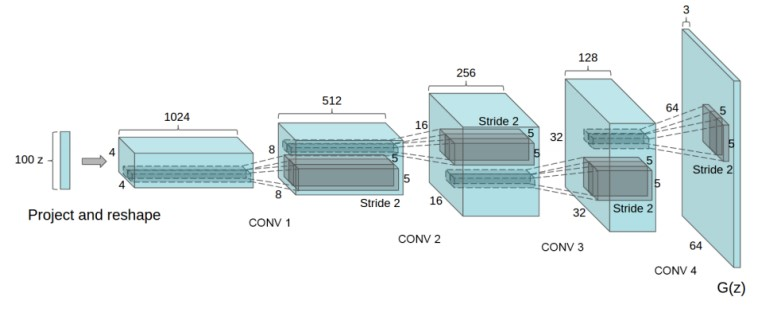
\includegraphics{wiki/3_1.jpg}
\caption{generator}
\end{figure}

    \hypertarget{cycle-gan-summary}{%
\subsection{1 Cycle GAN Summary}\label{cycle-gan-summary}}

CycleGAN is an image to image translation tasks that works when paired
label image for input dataset is not available. Previous models in image
to image translation task such as Pix2Pix needs paired label as they try
to find a one to one mapping between each pair but CycleGAN omitted this
need by trying to first learning a map from X to Y and then forcing
network to be able to construct input image which means learning a map
from Y to X and this is the cycle in CycleGAN name.

As we know in GANs there is a generator and a discriminator (standard
models) where generator tries to create images based on what mapping it
learned and the duty of discriminator is to distinguish between images
which being generated by the generator and real images from dataset.
Both networks are trained simultaneously. When training finished,
generator model learned the underlying distribution of data and can
create new images that are similar to dataset in term of style.

But there is flaw in the aforementioned approach. In simplified works
generator can learn only a mapping from a group of input images that
causes discriminator not to be able to classify fake images from real
ones and generator produces same images all the time no matter what
input is. Actually, generator discard input image and discriminator
fails on particular images and loss function still decreasing as no
constraintion violated.

The idea of forcing network to learn a reverse mapping from Y to X in
CycleGAN cause the loss to incorporate the reconstruction of input image
to be similar at the end.

G1(x) = y, G2(y)=z ---\textgreater{} x = z

The above notations says that if a generator cannot obtain input image
from the generated image from the original generator, the loss should be
high. Here is the network architecture:

\begin{figure}
\centering
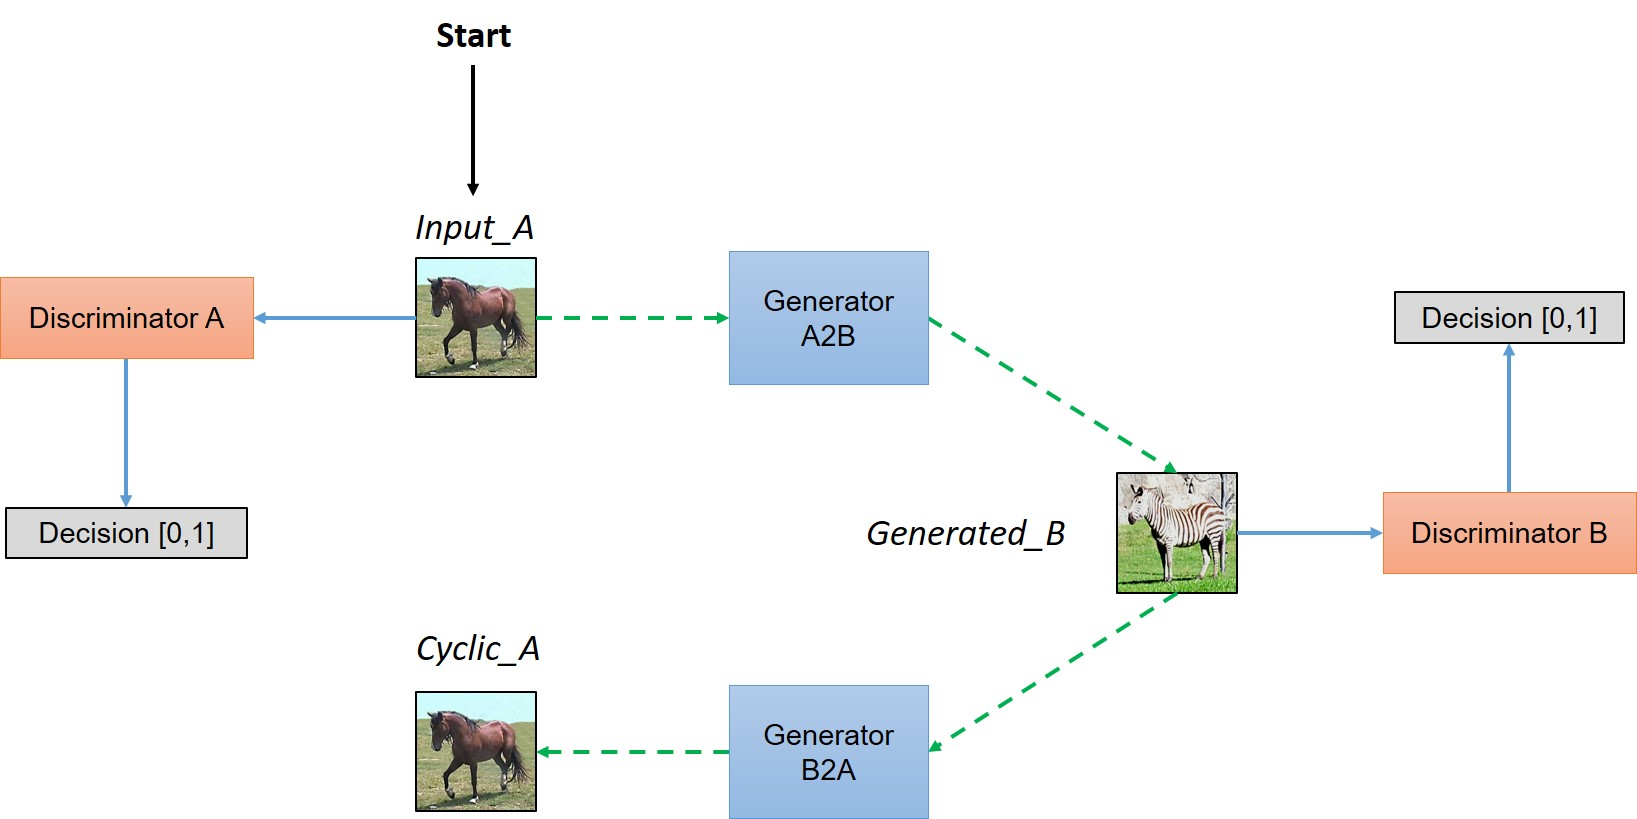
\includegraphics{wiki/3_5.jpg}
\caption{CycleGAN arch}
\end{figure}

Based on the architecture CycleGAN model works in this way:

First input image \texttt{img} is fed to first generator called
\texttt{g1} and \texttt{g1} tries to map \texttt{img} to another image
called \texttt{gen}. \texttt{g1} is learning a map from domain
\texttt{dm1} which is for \texttt{img} to domain \texttt{dm2} which
stands for \texttt{gen}. Now as we do not have any paired image in
dataset, we cannot ensure that \texttt{dm2} is meaningful which means
the mapping learned by \texttt{g1} can be anything. So to ensure about
it, the new generated image \texttt{g1} is fed to another generator
\texttt{g2} (where is the reverse of \texttt{g1} when trained) to
convert back \texttt{gen} to image \texttt{img}. This forces the model
to learn only the meaningful domain represented by the input
\texttt{img}. Also there are two discriminator, one for each generator
to enforce each generator to work well in theirs single task
transformation. In other words, discriminators try to enforce two
objectives: 1. Generators generate images similar to real data by
generating meaningful images 2. By generating images similar to input.

Here is image of CycleGAN with implementation terms:

\begin{figure}
\centering
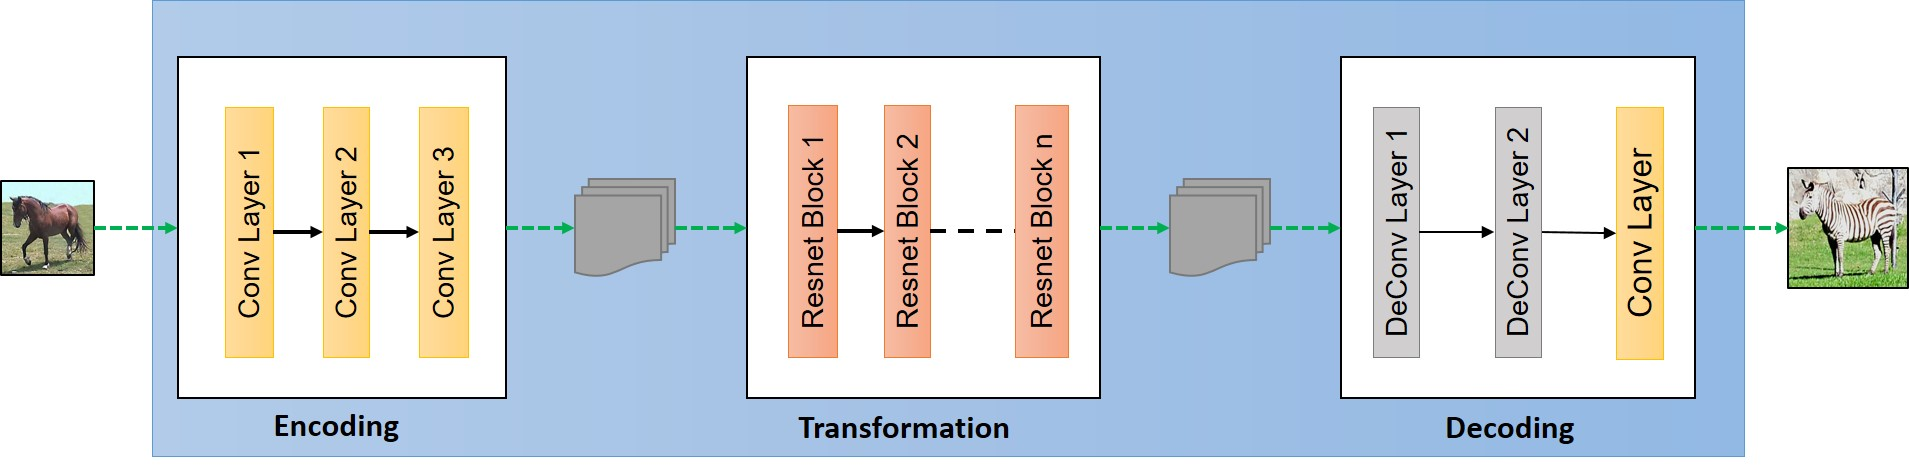
\includegraphics{wiki/3_6.jpg}
\caption{CycleGAN implem}
\end{figure}

Loss function needs to meet following constraints:

\begin{verbatim}
1. Discriminator must approve all the original images
2. Discriminator must reject all the images which are generated by corresponding Generators
3. Generators must make the discriminators approve all the generated images
4. The generated image must retain the property of original image, let's say if we get `gen` from `img` by `g1`, we must be able to get `img` by feeding `gen` to `g2`
\end{verbatim}

Both discriminators want to decreas their loss regarding their real
input images \texttt{D1(a)} and \texttt{D2(a)} Both discriminators want
to predict 0 for generated images so D wants to maximize
\texttt{D1(G2(b))} and \texttt{D2(G1(a))} Both generators want to fool
their discriminators so G wants to minimize \texttt{D2(G1(a))} and
\texttt{D1(G2(b))} And cycle loss that enables network the generate
images similar to their inputs which means the difference between input
image to a generator and its output should be small as possible so we
want to minimize \texttt{mean(a-ab,\ b-ba)} where \texttt{ab} is the
output of giving \texttt{a} to \texttt{g1} then \texttt{g2} and
\texttt{ba} in reverse manner.

    \hypertarget{answer-these-questions-about-pca-and-autoencoders}{%
\subsection{2 Answer these questions about PCA and
AutoEncoders:}\label{answer-these-questions-about-pca-and-autoencoders}}

\begin{enumerate}
\def\labelenumi{\arabic{enumi}.}
\tightlist
\item
  Supervision aspect.
\item
  Trainable aspect.
\item
  Compare from other aspects too.
\end{enumerate}

    \hypertarget{a-supervision}{%
\subsubsection{2.A Supervision}\label{a-supervision}}

In PCA only features (X) are needed as the only computations are eigen
values and coovariance matrix. But about Autoencoders it can be both
supervised or unsupervised depending on task but generally and as what
see in main AutoEncoders, they are unsupervised as they used to find
hidden structure in given data distributions.

    \hypertarget{b-trianable}{%
\subsubsection{2.B Trianable}\label{b-trianable}}

PCA uses eigen values and eigen vectors to find most dominant factors in
given data and then just transform them into new axis system using
orthogonal transforms so it is not trainable. But AutoEncoders are
neural network architectures that use optimizer to train model
iteratively.

    \hypertarget{c-other-aspects}{%
\subsubsection{2.C Other Aspects}\label{c-other-aspects}}

First thing about PCA is that it only works on data where features are
\textbf{linearly coorelated} to each other which for most of the tasks
in real world it fails. But on the other hand, AutoEncoders uses conv
(or fc) layers and non-linearity among them which enables it capture
almost any type of corelation between two arbitrary features and based
on the pattern recognition theorem, the capacity of AutoEncoders are
unlimited which means they can learn any kind of corelations but the
appropriate config needs to be found which is complex in practice.

\begin{figure}
\centering
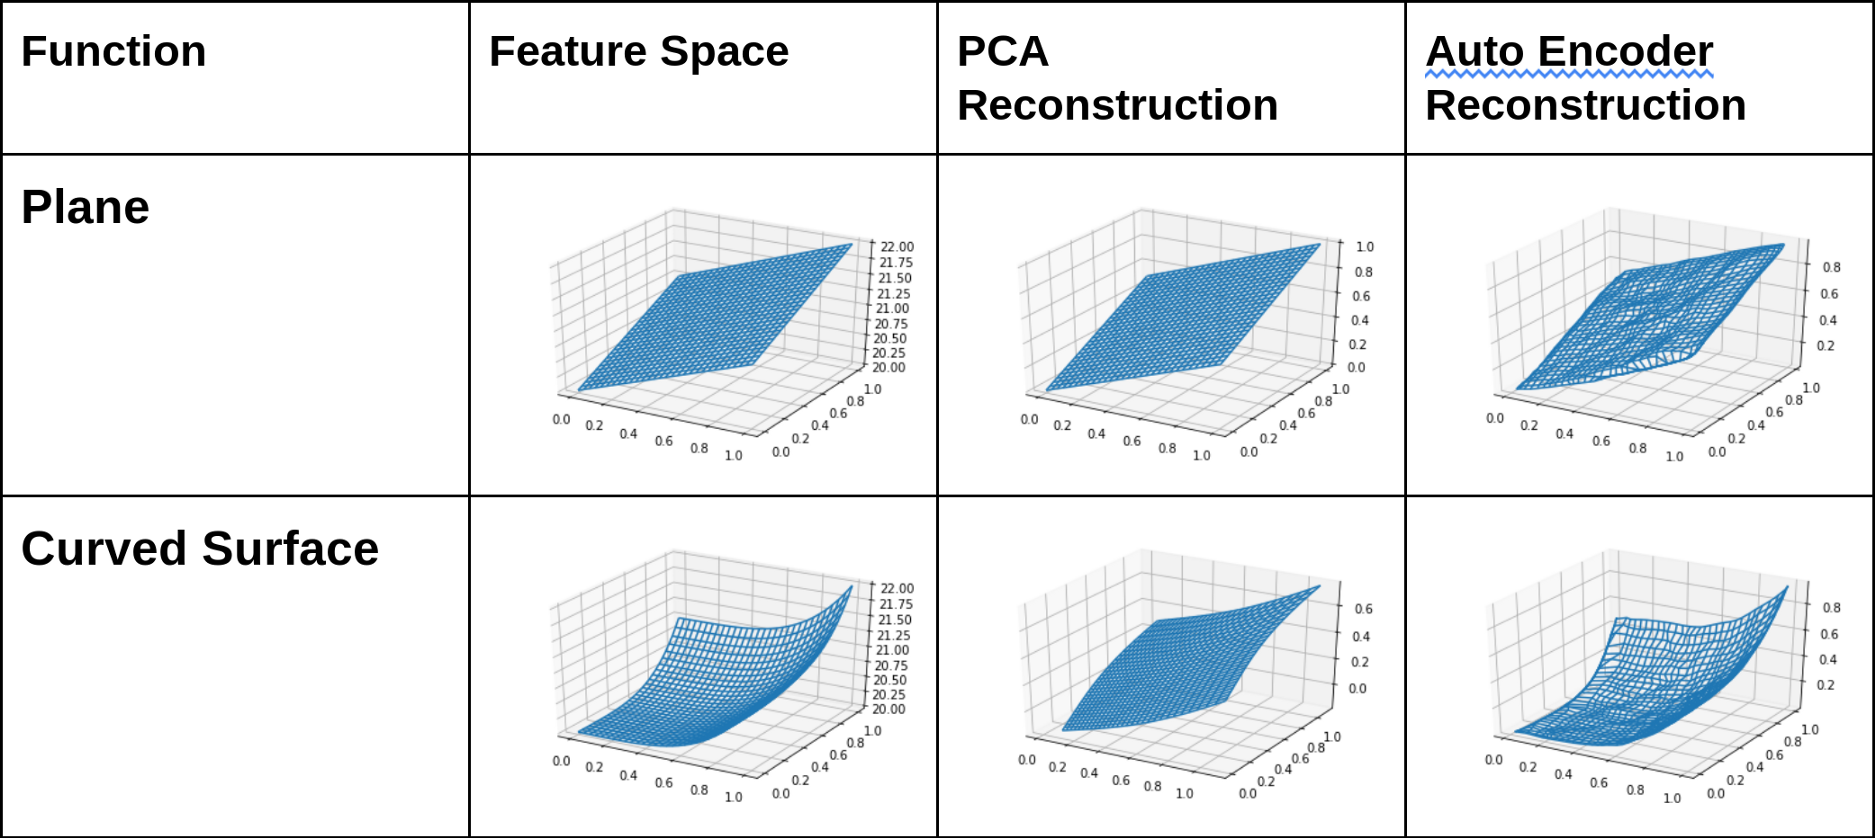
\includegraphics{wiki/2_1.png}
\caption{pca vs ae}
\end{figure}

About similarities, they both can find correlations in features so we
can skip some of features and use the **dimensionality reduction* aspect
of these two approaches.

About computations, as we know that PCA is linear and AutoEncoder is
non-linear, and PCA is not trainable and iterative but AutoEncoder is,
so it can be obtained that AutoEncoder needs much more computational
power and time.

Finding correct config for AutoEncoders is hard and almost there is no
fixed approach in general and it have to be learned for different data
distributins while PCA only uses statistical features of data and no
configuration is needed.

    \hypertarget{train-a-gan-network}{%
\subsection{3 Train a GAN Network}\label{train-a-gan-network}}

\begin{enumerate}
\def\labelenumi{\arabic{enumi}.}
\tightlist
\item
  Import Library
\item
  Set Hyperparameters
\item
  Load Data
\item
  Generator
\item
  Discriminator
\item
  Compile Models
\item
  Train Model
\end{enumerate}

\begin{figure}
\centering
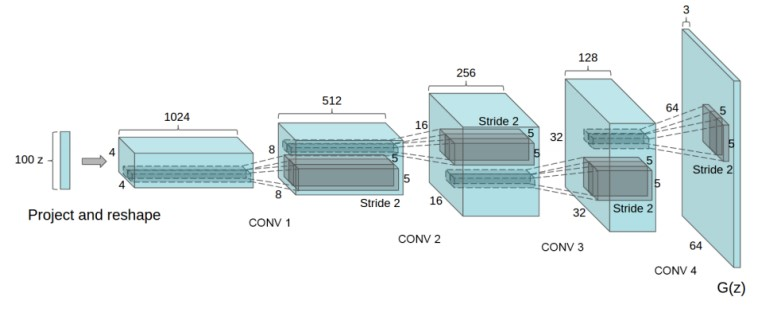
\includegraphics{wiki/3_1.jpg}
\caption{generator}
\end{figure}

    \_** NOTE: in my experiments using 1024 channels in the first layer of
generator hinders model to learn anything within 100 30 epochs so I
changed it to smaller value such as 256 and model learned much better
even in 5 epochs. **\_

\begin{figure}
\centering
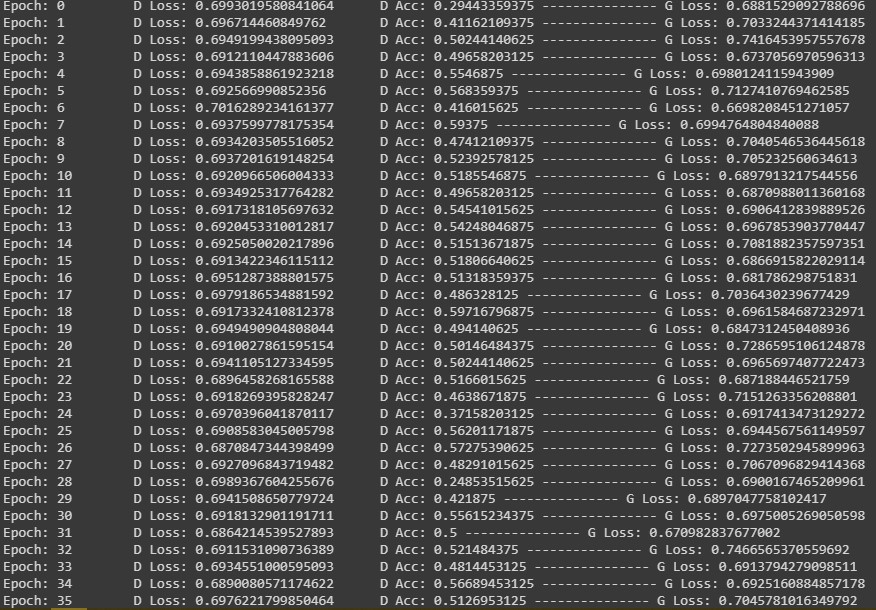
\includegraphics{wiki/3_2.jpg}
\caption{train fail on 1024}
\end{figure}

Trained generator after 30 epoch with 1024 channels:

\begin{figure}
\centering
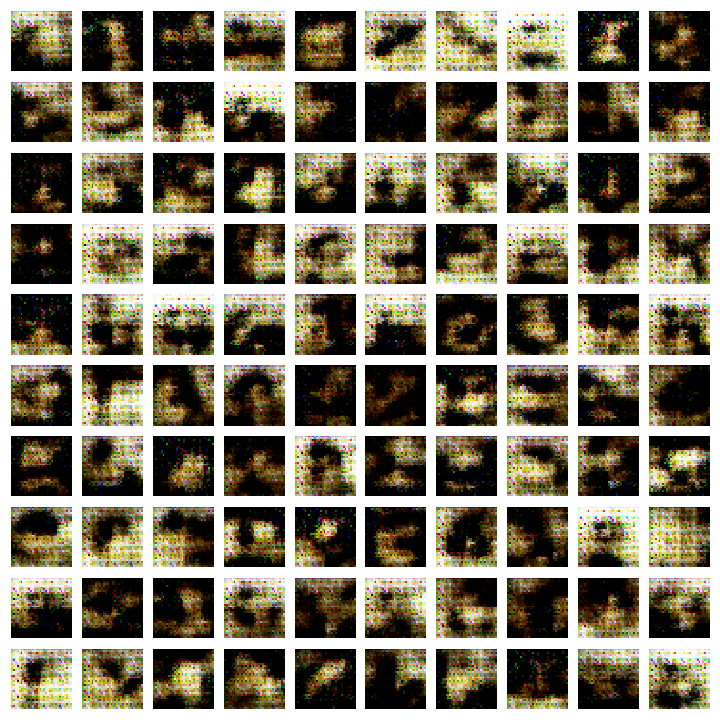
\includegraphics{wiki/3_3.png}
\caption{output 30 epoch 1024}
\end{figure}

Trained generator after 30 epoch with 256 channels:

\begin{figure}
\centering
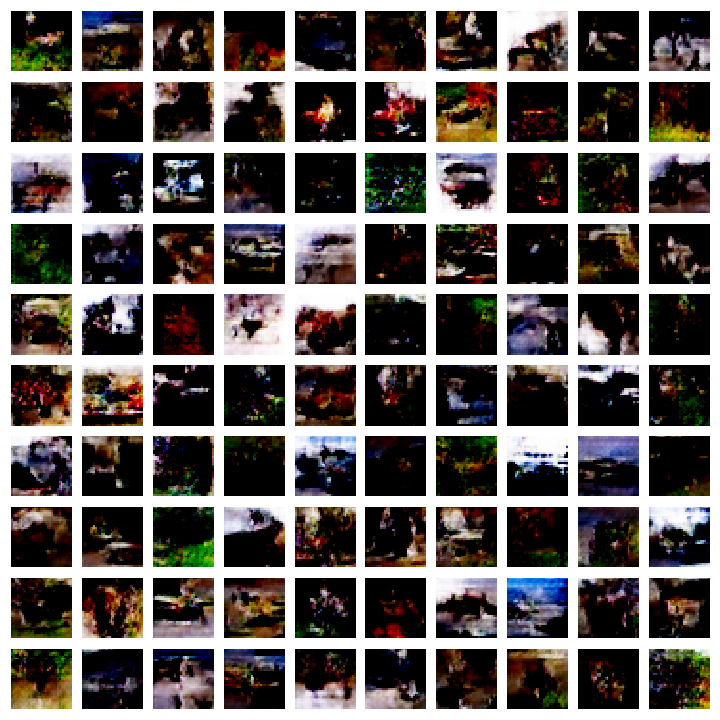
\includegraphics{wiki/3_4.png}
\caption{output 30 epoch 256}
\end{figure}

    \hypertarget{a-import-library}{%
\subsubsection{3.A Import Library}\label{a-import-library}}

    \begin{Verbatim}[commandchars=\\\{\}]
{\color{incolor}In [{\color{incolor} }]:} \PY{o}{\PYZpc{}}\PY{k}{tensorflow\PYZus{}version} 1.x
        
        \PY{k+kn}{import} \PY{n+nn}{os}
        
        \PY{k+kn}{import} \PY{n+nn}{matplotlib}\PY{n+nn}{.}\PY{n+nn}{pyplot} \PY{k}{as} \PY{n+nn}{plt}
        \PY{k+kn}{import} \PY{n+nn}{numpy} \PY{k}{as} \PY{n+nn}{np}
        
        \PY{k+kn}{from} \PY{n+nn}{keras}\PY{n+nn}{.}\PY{n+nn}{datasets} \PY{k}{import} \PY{n}{cifar10}
        \PY{k+kn}{from} \PY{n+nn}{keras}\PY{n+nn}{.}\PY{n+nn}{layers} \PY{k}{import} \PY{n}{Activation}
        \PY{k+kn}{from} \PY{n+nn}{keras}\PY{n+nn}{.}\PY{n+nn}{layers}\PY{n+nn}{.}\PY{n+nn}{advanced\PYZus{}activations} \PY{k}{import} \PY{n}{LeakyReLU}
        \PY{k+kn}{from} \PY{n+nn}{keras} \PY{k}{import} \PY{n}{initializers}
        \PY{k+kn}{from} \PY{n+nn}{keras}\PY{n+nn}{.}\PY{n+nn}{layers} \PY{k}{import} \PY{p}{(}\PY{n}{BatchNormalization}\PY{p}{,} \PY{n}{Conv2D}\PY{p}{,} \PY{n}{Conv2DTranspose}\PY{p}{,} \PY{n}{Dense}\PY{p}{,}
                                  \PY{n}{Dropout}\PY{p}{,} \PY{n}{Flatten}\PY{p}{,} \PY{n}{Input}\PY{p}{,} \PY{n}{Reshape}\PY{p}{,} \PY{n}{UpSampling2D}\PY{p}{,}
                                  \PY{n}{ZeroPadding2D}\PY{p}{)}
        \PY{k+kn}{from} \PY{n+nn}{keras}\PY{n+nn}{.}\PY{n+nn}{layers}\PY{n+nn}{.}\PY{n+nn}{advanced\PYZus{}activations} \PY{k}{import} \PY{n}{LeakyReLU}
        \PY{k+kn}{from} \PY{n+nn}{keras}\PY{n+nn}{.}\PY{n+nn}{models} \PY{k}{import} \PY{n}{Model}\PY{p}{,} \PY{n}{Sequential}
        \PY{k+kn}{from} \PY{n+nn}{keras}\PY{n+nn}{.}\PY{n+nn}{optimizers} \PY{k}{import} \PY{n}{Adam}
        
        \PY{k+kn}{from} \PY{n+nn}{PIL} \PY{k}{import} \PY{n}{Image}\PY{p}{,} \PY{n}{ImageDraw}
\end{Verbatim}


    \hypertarget{b-set-hyperparameters}{%
\subsubsection{3.B Set Hyperparameters}\label{b-set-hyperparameters}}

    \begin{Verbatim}[commandchars=\\\{\}]
{\color{incolor}In [{\color{incolor} }]:} \PY{n}{latent\PYZus{}dim} \PY{o}{=} \PY{l+m+mi}{100}
        
        \PY{n}{batch\PYZus{}size} \PY{o}{=} \PY{l+m+mi}{256}
        \PY{n}{epochs} \PY{o}{=} \PY{l+m+mi}{200}
        
        \PY{n}{img\PYZus{}rows} \PY{o}{=} \PY{l+m+mi}{32}
        \PY{n}{img\PYZus{}cols} \PY{o}{=} \PY{l+m+mi}{32}
        \PY{n}{channels} \PY{o}{=} \PY{l+m+mi}{3}
        \PY{n}{kernel\PYZus{}size} \PY{o}{=} \PY{l+m+mi}{3}
        
        \PY{n}{save\PYZus{}path} \PY{o}{=} \PY{l+s+s1}{\PYZsq{}}\PY{l+s+s1}{model}\PY{l+s+s1}{\PYZsq{}}
        
        \PY{n}{img\PYZus{}rows}\PY{p}{,} \PY{n}{img\PYZus{}cols}\PY{p}{,} \PY{n}{channels} \PY{o}{=} \PY{l+m+mi}{32}\PY{p}{,} \PY{l+m+mi}{32}\PY{p}{,} \PY{l+m+mi}{3}
        \PY{n}{img\PYZus{}shape} \PY{o}{=} \PY{p}{(}\PY{n}{img\PYZus{}rows}\PY{p}{,} \PY{n}{img\PYZus{}cols}\PY{p}{,} \PY{n}{channels}\PY{p}{)}
        
        \PY{n}{optimizer} \PY{o}{=} \PY{n}{Adam}\PY{p}{(}\PY{l+m+mf}{0.0002}\PY{p}{,} \PY{l+m+mf}{0.5}\PY{p}{)}
        
        \PY{k}{if} \PY{o+ow}{not} \PY{n}{os}\PY{o}{.}\PY{n}{path}\PY{o}{.}\PY{n}{isdir}\PY{p}{(}\PY{n}{save\PYZus{}path}\PY{p}{)}\PY{p}{:}
            \PY{n}{os}\PY{o}{.}\PY{n}{mkdir}\PY{p}{(}\PY{n}{save\PYZus{}path}\PY{p}{)}
\end{Verbatim}


    \hypertarget{c-load-data}{%
\subsubsection{3.C Load Data}\label{c-load-data}}

    \begin{Verbatim}[commandchars=\\\{\}]
{\color{incolor}In [{\color{incolor}23}]:} \PY{p}{(}\PY{n}{x\PYZus{}train}\PY{p}{,} \PY{n}{y\PYZus{}train}\PY{p}{)}\PY{p}{,} \PY{p}{(}\PY{n}{x\PYZus{}test}\PY{p}{,} \PY{n}{y\PYZus{}test}\PY{p}{)} \PY{o}{=} \PY{n}{cifar10}\PY{o}{.}\PY{n}{load\PYZus{}data}\PY{p}{(}\PY{p}{)}
         \PY{n}{x\PYZus{}train} \PY{o}{=} \PY{p}{(}\PY{n}{x\PYZus{}train}\PY{o}{.}\PY{n}{astype}\PY{p}{(}\PY{n}{np}\PY{o}{.}\PY{n}{float32}\PY{p}{)} \PY{o}{\PYZhy{}} \PY{l+m+mf}{127.5}\PY{p}{)} \PY{o}{/} \PY{l+m+mf}{127.5}
         \PY{n+nb}{print}\PY{p}{(}\PY{n}{x\PYZus{}train}\PY{o}{.}\PY{n}{shape}\PY{p}{)}
\end{Verbatim}


    \begin{Verbatim}[commandchars=\\\{\}]
(50000, 32, 32, 3)

    \end{Verbatim}

    \hypertarget{d-generator}{%
\subsubsection{3.D Generator}\label{d-generator}}

    \begin{Verbatim}[commandchars=\\\{\}]
{\color{incolor}In [{\color{incolor}24}]:} \PY{k}{def} \PY{n+nf}{create\PYZus{}generator}\PY{p}{(}\PY{p}{)}\PY{p}{:}
             \PY{n}{model} \PY{o}{=} \PY{n}{Sequential}\PY{p}{(}\PY{p}{)}
             
             \PY{n}{model}\PY{o}{.}\PY{n}{add}\PY{p}{(}\PY{n}{Dense}\PY{p}{(}\PY{l+m+mi}{256} \PY{o}{*} \PY{l+m+mi}{4} \PY{o}{*} \PY{l+m+mi}{4}\PY{p}{,} \PY{n}{input\PYZus{}shape}\PY{o}{=}\PY{p}{(}\PY{n}{latent\PYZus{}dim}\PY{p}{,}\PY{p}{)}\PY{p}{)}\PY{p}{)}
             \PY{n}{model}\PY{o}{.}\PY{n}{add}\PY{p}{(}\PY{n}{LeakyReLU}\PY{p}{(}\PY{n}{alpha}\PY{o}{=}\PY{l+m+mf}{0.2}\PY{p}{)}\PY{p}{)}
             \PY{n}{model}\PY{o}{.}\PY{n}{add}\PY{p}{(}\PY{n}{Reshape}\PY{p}{(}\PY{p}{(}\PY{l+m+mi}{4}\PY{p}{,} \PY{l+m+mi}{4}\PY{p}{,} \PY{l+m+mi}{256}\PY{p}{)}\PY{p}{)}\PY{p}{)}
         
             \PY{n}{model}\PY{o}{.}\PY{n}{add}\PY{p}{(}\PY{n}{Conv2DTranspose}\PY{p}{(}\PY{l+m+mi}{1024}\PY{p}{,} \PY{n}{kernel\PYZus{}size}\PY{o}{=}\PY{p}{(}\PY{l+m+mi}{2}\PY{p}{,} \PY{l+m+mi}{2}\PY{p}{)}\PY{p}{,} \PY{n}{padding}\PY{o}{=}\PY{l+s+s1}{\PYZsq{}}\PY{l+s+s1}{same}\PY{l+s+s1}{\PYZsq{}}\PY{p}{)}\PY{p}{)}
             \PY{n}{model}\PY{o}{.}\PY{n}{add}\PY{p}{(}\PY{n}{LeakyReLU}\PY{p}{(}\PY{n}{alpha}\PY{o}{=}\PY{l+m+mf}{0.2}\PY{p}{)}\PY{p}{)}
         
             \PY{n}{model}\PY{o}{.}\PY{n}{add}\PY{p}{(}\PY{n}{Conv2DTranspose}\PY{p}{(}\PY{l+m+mi}{128}\PY{p}{,} \PY{n}{kernel\PYZus{}size}\PY{o}{=}\PY{p}{(}\PY{l+m+mi}{2}\PY{p}{,} \PY{l+m+mi}{2}\PY{p}{)}\PY{p}{,} \PY{n}{strides}\PY{o}{=}\PY{l+m+mi}{2}\PY{p}{,} \PY{n}{padding}\PY{o}{=}\PY{l+s+s1}{\PYZsq{}}\PY{l+s+s1}{same}\PY{l+s+s1}{\PYZsq{}}\PY{p}{)}\PY{p}{)}
             \PY{n}{model}\PY{o}{.}\PY{n}{add}\PY{p}{(}\PY{n}{LeakyReLU}\PY{p}{(}\PY{n}{alpha}\PY{o}{=}\PY{l+m+mf}{0.2}\PY{p}{)}\PY{p}{)}
             
             \PY{n}{model}\PY{o}{.}\PY{n}{add}\PY{p}{(}\PY{n}{Conv2DTranspose}\PY{p}{(}\PY{l+m+mi}{128}\PY{p}{,} \PY{n}{kernel\PYZus{}size}\PY{o}{=}\PY{p}{(}\PY{l+m+mi}{2}\PY{p}{,} \PY{l+m+mi}{2}\PY{p}{)}\PY{p}{,} \PY{n}{strides}\PY{o}{=}\PY{l+m+mi}{2}\PY{p}{,} \PY{n}{padding}\PY{o}{=}\PY{l+s+s1}{\PYZsq{}}\PY{l+s+s1}{same}\PY{l+s+s1}{\PYZsq{}}\PY{p}{)}\PY{p}{)}
             \PY{n}{model}\PY{o}{.}\PY{n}{add}\PY{p}{(}\PY{n}{LeakyReLU}\PY{p}{(}\PY{n}{alpha}\PY{o}{=}\PY{l+m+mf}{0.2}\PY{p}{)}\PY{p}{)}
         
             \PY{n}{model}\PY{o}{.}\PY{n}{add}\PY{p}{(}\PY{n}{Conv2DTranspose}\PY{p}{(}\PY{l+m+mi}{64}\PY{p}{,} \PY{n}{kernel\PYZus{}size}\PY{o}{=}\PY{p}{(}\PY{l+m+mi}{2}\PY{p}{,} \PY{l+m+mi}{2}\PY{p}{)}\PY{p}{,} \PY{n}{strides}\PY{o}{=}\PY{l+m+mi}{2}\PY{p}{,} \PY{n}{padding}\PY{o}{=}\PY{l+s+s1}{\PYZsq{}}\PY{l+s+s1}{same}\PY{l+s+s1}{\PYZsq{}}\PY{p}{)}\PY{p}{)}
             \PY{n}{model}\PY{o}{.}\PY{n}{add}\PY{p}{(}\PY{n}{LeakyReLU}\PY{p}{(}\PY{n}{alpha}\PY{o}{=}\PY{l+m+mf}{0.2}\PY{p}{)}\PY{p}{)}
         
             \PY{n}{model}\PY{o}{.}\PY{n}{add}\PY{p}{(}\PY{n}{Conv2DTranspose}\PY{p}{(}\PY{l+m+mi}{3}\PY{p}{,} \PY{n}{kernel\PYZus{}size}\PY{o}{=}\PY{p}{(}\PY{l+m+mi}{2}\PY{p}{,} \PY{l+m+mi}{2}\PY{p}{)}\PY{p}{,} \PY{n}{strides}\PY{o}{=}\PY{l+m+mi}{1}\PY{p}{,} \PY{n}{padding}\PY{o}{=}\PY{l+s+s1}{\PYZsq{}}\PY{l+s+s1}{same}\PY{l+s+s1}{\PYZsq{}}\PY{p}{)}\PY{p}{)}
             \PY{n}{model}\PY{o}{.}\PY{n}{add}\PY{p}{(}\PY{n}{Activation}\PY{p}{(}\PY{l+s+s1}{\PYZsq{}}\PY{l+s+s1}{tanh}\PY{l+s+s1}{\PYZsq{}}\PY{p}{)}\PY{p}{)}
             
             \PY{n}{model}\PY{o}{.}\PY{n}{compile}\PY{p}{(}\PY{n}{loss}\PY{o}{=}\PY{l+s+s1}{\PYZsq{}}\PY{l+s+s1}{binary\PYZus{}crossentropy}\PY{l+s+s1}{\PYZsq{}}\PY{p}{,} \PY{n}{optimizer}\PY{o}{=}\PY{n}{optimizer}\PY{p}{,} \PY{n}{metrics}\PY{o}{=}\PY{p}{[}\PY{l+s+s1}{\PYZsq{}}\PY{l+s+s1}{accuracy}\PY{l+s+s1}{\PYZsq{}}\PY{p}{]}\PY{p}{)}
             \PY{k}{return} \PY{n}{model}
         \PY{n}{generator} \PY{o}{=} \PY{n}{create\PYZus{}generator}\PY{p}{(}\PY{p}{)}
         \PY{n}{generator}\PY{o}{.}\PY{n}{summary}\PY{p}{(}\PY{p}{)}
         
         \PY{c+c1}{\PYZsh{} note as my dataset images are 32x32, I changed last layer of generator to output 32x32}
         \PY{c+c1}{\PYZsh{} as interpolating this size to 64x64 is not good for training a small model like this on low epochs.}
\end{Verbatim}


    \begin{Verbatim}[commandchars=\\\{\}]
Model: "sequential\_6"
\_\_\_\_\_\_\_\_\_\_\_\_\_\_\_\_\_\_\_\_\_\_\_\_\_\_\_\_\_\_\_\_\_\_\_\_\_\_\_\_\_\_\_\_\_\_\_\_\_\_\_\_\_\_\_\_\_\_\_\_\_\_\_\_\_
Layer (type)                 Output Shape              Param \#   
=================================================================
dense\_6 (Dense)              (None, 4096)              413696    
\_\_\_\_\_\_\_\_\_\_\_\_\_\_\_\_\_\_\_\_\_\_\_\_\_\_\_\_\_\_\_\_\_\_\_\_\_\_\_\_\_\_\_\_\_\_\_\_\_\_\_\_\_\_\_\_\_\_\_\_\_\_\_\_\_
leaky\_re\_lu\_26 (LeakyReLU)   (None, 4096)              0         
\_\_\_\_\_\_\_\_\_\_\_\_\_\_\_\_\_\_\_\_\_\_\_\_\_\_\_\_\_\_\_\_\_\_\_\_\_\_\_\_\_\_\_\_\_\_\_\_\_\_\_\_\_\_\_\_\_\_\_\_\_\_\_\_\_
reshape\_4 (Reshape)          (None, 4, 4, 256)         0         
\_\_\_\_\_\_\_\_\_\_\_\_\_\_\_\_\_\_\_\_\_\_\_\_\_\_\_\_\_\_\_\_\_\_\_\_\_\_\_\_\_\_\_\_\_\_\_\_\_\_\_\_\_\_\_\_\_\_\_\_\_\_\_\_\_
conv2d\_transpose\_16 (Conv2DT (None, 4, 4, 1024)        1049600   
\_\_\_\_\_\_\_\_\_\_\_\_\_\_\_\_\_\_\_\_\_\_\_\_\_\_\_\_\_\_\_\_\_\_\_\_\_\_\_\_\_\_\_\_\_\_\_\_\_\_\_\_\_\_\_\_\_\_\_\_\_\_\_\_\_
leaky\_re\_lu\_27 (LeakyReLU)   (None, 4, 4, 1024)        0         
\_\_\_\_\_\_\_\_\_\_\_\_\_\_\_\_\_\_\_\_\_\_\_\_\_\_\_\_\_\_\_\_\_\_\_\_\_\_\_\_\_\_\_\_\_\_\_\_\_\_\_\_\_\_\_\_\_\_\_\_\_\_\_\_\_
conv2d\_transpose\_17 (Conv2DT (None, 8, 8, 128)         524416    
\_\_\_\_\_\_\_\_\_\_\_\_\_\_\_\_\_\_\_\_\_\_\_\_\_\_\_\_\_\_\_\_\_\_\_\_\_\_\_\_\_\_\_\_\_\_\_\_\_\_\_\_\_\_\_\_\_\_\_\_\_\_\_\_\_
leaky\_re\_lu\_28 (LeakyReLU)   (None, 8, 8, 128)         0         
\_\_\_\_\_\_\_\_\_\_\_\_\_\_\_\_\_\_\_\_\_\_\_\_\_\_\_\_\_\_\_\_\_\_\_\_\_\_\_\_\_\_\_\_\_\_\_\_\_\_\_\_\_\_\_\_\_\_\_\_\_\_\_\_\_
conv2d\_transpose\_18 (Conv2DT (None, 16, 16, 128)       65664     
\_\_\_\_\_\_\_\_\_\_\_\_\_\_\_\_\_\_\_\_\_\_\_\_\_\_\_\_\_\_\_\_\_\_\_\_\_\_\_\_\_\_\_\_\_\_\_\_\_\_\_\_\_\_\_\_\_\_\_\_\_\_\_\_\_
leaky\_re\_lu\_29 (LeakyReLU)   (None, 16, 16, 128)       0         
\_\_\_\_\_\_\_\_\_\_\_\_\_\_\_\_\_\_\_\_\_\_\_\_\_\_\_\_\_\_\_\_\_\_\_\_\_\_\_\_\_\_\_\_\_\_\_\_\_\_\_\_\_\_\_\_\_\_\_\_\_\_\_\_\_
conv2d\_transpose\_19 (Conv2DT (None, 32, 32, 64)        32832     
\_\_\_\_\_\_\_\_\_\_\_\_\_\_\_\_\_\_\_\_\_\_\_\_\_\_\_\_\_\_\_\_\_\_\_\_\_\_\_\_\_\_\_\_\_\_\_\_\_\_\_\_\_\_\_\_\_\_\_\_\_\_\_\_\_
leaky\_re\_lu\_30 (LeakyReLU)   (None, 32, 32, 64)        0         
\_\_\_\_\_\_\_\_\_\_\_\_\_\_\_\_\_\_\_\_\_\_\_\_\_\_\_\_\_\_\_\_\_\_\_\_\_\_\_\_\_\_\_\_\_\_\_\_\_\_\_\_\_\_\_\_\_\_\_\_\_\_\_\_\_
conv2d\_transpose\_20 (Conv2DT (None, 32, 32, 3)         771       
\_\_\_\_\_\_\_\_\_\_\_\_\_\_\_\_\_\_\_\_\_\_\_\_\_\_\_\_\_\_\_\_\_\_\_\_\_\_\_\_\_\_\_\_\_\_\_\_\_\_\_\_\_\_\_\_\_\_\_\_\_\_\_\_\_
activation\_4 (Activation)    (None, 32, 32, 3)         0         
=================================================================
Total params: 2,086,979
Trainable params: 2,086,979
Non-trainable params: 0
\_\_\_\_\_\_\_\_\_\_\_\_\_\_\_\_\_\_\_\_\_\_\_\_\_\_\_\_\_\_\_\_\_\_\_\_\_\_\_\_\_\_\_\_\_\_\_\_\_\_\_\_\_\_\_\_\_\_\_\_\_\_\_\_\_

    \end{Verbatim}

    \hypertarget{e-discriminator}{%
\subsubsection{3.E Discriminator}\label{e-discriminator}}

    \begin{Verbatim}[commandchars=\\\{\}]
{\color{incolor}In [{\color{incolor}25}]:} \PY{k}{def} \PY{n+nf}{create\PYZus{}descriminator}\PY{p}{(}\PY{p}{)}\PY{p}{:}
             \PY{n}{model} \PY{o}{=} \PY{n}{Sequential}\PY{p}{(}\PY{p}{)}
             
             \PY{n}{model}\PY{o}{.}\PY{n}{add}\PY{p}{(}\PY{n}{Conv2D}\PY{p}{(}\PY{l+m+mi}{32}\PY{p}{,} \PY{n}{kernel\PYZus{}size}\PY{o}{=}\PY{n}{kernel\PYZus{}size}\PY{p}{,} \PY{n}{strides}\PY{o}{=}\PY{l+m+mi}{2}\PY{p}{,} \PY{n}{input\PYZus{}shape}\PY{o}{=}\PY{n}{img\PYZus{}shape}\PY{p}{,} \PY{n}{padding}\PY{o}{=}\PY{l+s+s2}{\PYZdq{}}\PY{l+s+s2}{same}\PY{l+s+s2}{\PYZdq{}}\PY{p}{)}\PY{p}{)}
             \PY{n}{model}\PY{o}{.}\PY{n}{add}\PY{p}{(}\PY{n}{LeakyReLU}\PY{p}{(}\PY{n}{alpha}\PY{o}{=}\PY{l+m+mf}{0.2}\PY{p}{)}\PY{p}{)}
             \PY{n}{model}\PY{o}{.}\PY{n}{add}\PY{p}{(}\PY{n}{Dropout}\PY{p}{(}\PY{l+m+mf}{0.25}\PY{p}{)}\PY{p}{)}
         
             \PY{n}{model}\PY{o}{.}\PY{n}{add}\PY{p}{(}\PY{n}{Conv2D}\PY{p}{(}\PY{l+m+mi}{64}\PY{p}{,} \PY{n}{kernel\PYZus{}size}\PY{o}{=}\PY{n}{kernel\PYZus{}size}\PY{p}{,} \PY{n}{strides}\PY{o}{=}\PY{l+m+mi}{2}\PY{p}{,} \PY{n}{padding}\PY{o}{=}\PY{l+s+s2}{\PYZdq{}}\PY{l+s+s2}{same}\PY{l+s+s2}{\PYZdq{}}\PY{p}{)}\PY{p}{)}
             \PY{n}{model}\PY{o}{.}\PY{n}{add}\PY{p}{(}\PY{n}{ZeroPadding2D}\PY{p}{(}\PY{n}{padding}\PY{o}{=}\PY{p}{(}\PY{p}{(}\PY{l+m+mi}{0}\PY{p}{,} \PY{l+m+mi}{1}\PY{p}{)}\PY{p}{,} \PY{p}{(}\PY{l+m+mi}{0}\PY{p}{,} \PY{l+m+mi}{1}\PY{p}{)}\PY{p}{)}\PY{p}{)}\PY{p}{)}
             \PY{n}{model}\PY{o}{.}\PY{n}{add}\PY{p}{(}\PY{n}{LeakyReLU}\PY{p}{(}\PY{n}{alpha}\PY{o}{=}\PY{l+m+mf}{0.2}\PY{p}{)}\PY{p}{)}
             \PY{n}{model}\PY{o}{.}\PY{n}{add}\PY{p}{(}\PY{n}{Dropout}\PY{p}{(}\PY{l+m+mf}{0.25}\PY{p}{)}\PY{p}{)}
         
             \PY{n}{model}\PY{o}{.}\PY{n}{add}\PY{p}{(}\PY{n}{Conv2D}\PY{p}{(}\PY{l+m+mi}{128}\PY{p}{,} \PY{n}{kernel\PYZus{}size}\PY{o}{=}\PY{n}{kernel\PYZus{}size}\PY{p}{,} \PY{n}{strides}\PY{o}{=}\PY{l+m+mi}{2}\PY{p}{,} \PY{n}{padding}\PY{o}{=}\PY{l+s+s2}{\PYZdq{}}\PY{l+s+s2}{same}\PY{l+s+s2}{\PYZdq{}}\PY{p}{)}\PY{p}{)}
             \PY{n}{model}\PY{o}{.}\PY{n}{add}\PY{p}{(}\PY{n}{LeakyReLU}\PY{p}{(}\PY{n}{alpha}\PY{o}{=}\PY{l+m+mf}{0.2}\PY{p}{)}\PY{p}{)}
             \PY{n}{model}\PY{o}{.}\PY{n}{add}\PY{p}{(}\PY{n}{Dropout}\PY{p}{(}\PY{l+m+mf}{0.25}\PY{p}{)}\PY{p}{)}
         
             \PY{n}{model}\PY{o}{.}\PY{n}{add}\PY{p}{(}\PY{n}{Conv2D}\PY{p}{(}\PY{l+m+mi}{256}\PY{p}{,} \PY{n}{kernel\PYZus{}size}\PY{o}{=}\PY{n}{kernel\PYZus{}size}\PY{p}{,} \PY{n}{strides}\PY{o}{=}\PY{l+m+mi}{1}\PY{p}{,} \PY{n}{padding}\PY{o}{=}\PY{l+s+s2}{\PYZdq{}}\PY{l+s+s2}{same}\PY{l+s+s2}{\PYZdq{}}\PY{p}{)}\PY{p}{)}
             \PY{n}{model}\PY{o}{.}\PY{n}{add}\PY{p}{(}\PY{n}{LeakyReLU}\PY{p}{(}\PY{n}{alpha}\PY{o}{=}\PY{l+m+mf}{0.2}\PY{p}{)}\PY{p}{)}
             \PY{n}{model}\PY{o}{.}\PY{n}{add}\PY{p}{(}\PY{n}{Dropout}\PY{p}{(}\PY{l+m+mf}{0.25}\PY{p}{)}\PY{p}{)}
         
             \PY{n}{model}\PY{o}{.}\PY{n}{add}\PY{p}{(}\PY{n}{Conv2D}\PY{p}{(}\PY{l+m+mi}{512}\PY{p}{,} \PY{n}{kernel\PYZus{}size}\PY{o}{=}\PY{n}{kernel\PYZus{}size}\PY{p}{,} \PY{n}{strides}\PY{o}{=}\PY{l+m+mi}{1}\PY{p}{,} \PY{n}{padding}\PY{o}{=}\PY{l+s+s2}{\PYZdq{}}\PY{l+s+s2}{same}\PY{l+s+s2}{\PYZdq{}}\PY{p}{)}\PY{p}{)}
             \PY{n}{model}\PY{o}{.}\PY{n}{add}\PY{p}{(}\PY{n}{LeakyReLU}\PY{p}{(}\PY{n}{alpha}\PY{o}{=}\PY{l+m+mf}{0.2}\PY{p}{)}\PY{p}{)}
             \PY{n}{model}\PY{o}{.}\PY{n}{add}\PY{p}{(}\PY{n}{Dropout}\PY{p}{(}\PY{l+m+mf}{0.25}\PY{p}{)}\PY{p}{)}
         
             \PY{n}{model}\PY{o}{.}\PY{n}{add}\PY{p}{(}\PY{n}{Flatten}\PY{p}{(}\PY{p}{)}\PY{p}{)}
             \PY{n}{model}\PY{o}{.}\PY{n}{add}\PY{p}{(}\PY{n}{Dense}\PY{p}{(}\PY{l+m+mi}{1}\PY{p}{,} \PY{n}{activation}\PY{o}{=}\PY{l+s+s1}{\PYZsq{}}\PY{l+s+s1}{sigmoid}\PY{l+s+s1}{\PYZsq{}}\PY{p}{)}\PY{p}{)}
             
             \PY{n}{model}\PY{o}{.}\PY{n}{compile}\PY{p}{(}\PY{n}{loss}\PY{o}{=}\PY{l+s+s1}{\PYZsq{}}\PY{l+s+s1}{binary\PYZus{}crossentropy}\PY{l+s+s1}{\PYZsq{}}\PY{p}{,} \PY{n}{optimizer}\PY{o}{=}\PY{n}{optimizer}\PY{p}{,} \PY{n}{metrics}\PY{o}{=}\PY{p}{[}\PY{l+s+s1}{\PYZsq{}}\PY{l+s+s1}{accuracy}\PY{l+s+s1}{\PYZsq{}}\PY{p}{]}\PY{p}{)}
             \PY{k}{return} \PY{n}{model}
         \PY{n}{discriminator} \PY{o}{=} \PY{n}{create\PYZus{}descriminator}\PY{p}{(}\PY{p}{)}
         \PY{n}{discriminator}\PY{o}{.}\PY{n}{summary}\PY{p}{(}\PY{p}{)}
\end{Verbatim}


    \begin{Verbatim}[commandchars=\\\{\}]
Model: "sequential\_7"
\_\_\_\_\_\_\_\_\_\_\_\_\_\_\_\_\_\_\_\_\_\_\_\_\_\_\_\_\_\_\_\_\_\_\_\_\_\_\_\_\_\_\_\_\_\_\_\_\_\_\_\_\_\_\_\_\_\_\_\_\_\_\_\_\_
Layer (type)                 Output Shape              Param \#   
=================================================================
conv2d\_11 (Conv2D)           (None, 16, 16, 32)        896       
\_\_\_\_\_\_\_\_\_\_\_\_\_\_\_\_\_\_\_\_\_\_\_\_\_\_\_\_\_\_\_\_\_\_\_\_\_\_\_\_\_\_\_\_\_\_\_\_\_\_\_\_\_\_\_\_\_\_\_\_\_\_\_\_\_
leaky\_re\_lu\_31 (LeakyReLU)   (None, 16, 16, 32)        0         
\_\_\_\_\_\_\_\_\_\_\_\_\_\_\_\_\_\_\_\_\_\_\_\_\_\_\_\_\_\_\_\_\_\_\_\_\_\_\_\_\_\_\_\_\_\_\_\_\_\_\_\_\_\_\_\_\_\_\_\_\_\_\_\_\_
dropout\_11 (Dropout)         (None, 16, 16, 32)        0         
\_\_\_\_\_\_\_\_\_\_\_\_\_\_\_\_\_\_\_\_\_\_\_\_\_\_\_\_\_\_\_\_\_\_\_\_\_\_\_\_\_\_\_\_\_\_\_\_\_\_\_\_\_\_\_\_\_\_\_\_\_\_\_\_\_
conv2d\_12 (Conv2D)           (None, 8, 8, 64)          18496     
\_\_\_\_\_\_\_\_\_\_\_\_\_\_\_\_\_\_\_\_\_\_\_\_\_\_\_\_\_\_\_\_\_\_\_\_\_\_\_\_\_\_\_\_\_\_\_\_\_\_\_\_\_\_\_\_\_\_\_\_\_\_\_\_\_
zero\_padding2d\_3 (ZeroPaddin (None, 9, 9, 64)          0         
\_\_\_\_\_\_\_\_\_\_\_\_\_\_\_\_\_\_\_\_\_\_\_\_\_\_\_\_\_\_\_\_\_\_\_\_\_\_\_\_\_\_\_\_\_\_\_\_\_\_\_\_\_\_\_\_\_\_\_\_\_\_\_\_\_
leaky\_re\_lu\_32 (LeakyReLU)   (None, 9, 9, 64)          0         
\_\_\_\_\_\_\_\_\_\_\_\_\_\_\_\_\_\_\_\_\_\_\_\_\_\_\_\_\_\_\_\_\_\_\_\_\_\_\_\_\_\_\_\_\_\_\_\_\_\_\_\_\_\_\_\_\_\_\_\_\_\_\_\_\_
dropout\_12 (Dropout)         (None, 9, 9, 64)          0         
\_\_\_\_\_\_\_\_\_\_\_\_\_\_\_\_\_\_\_\_\_\_\_\_\_\_\_\_\_\_\_\_\_\_\_\_\_\_\_\_\_\_\_\_\_\_\_\_\_\_\_\_\_\_\_\_\_\_\_\_\_\_\_\_\_
conv2d\_13 (Conv2D)           (None, 5, 5, 128)         73856     
\_\_\_\_\_\_\_\_\_\_\_\_\_\_\_\_\_\_\_\_\_\_\_\_\_\_\_\_\_\_\_\_\_\_\_\_\_\_\_\_\_\_\_\_\_\_\_\_\_\_\_\_\_\_\_\_\_\_\_\_\_\_\_\_\_
leaky\_re\_lu\_33 (LeakyReLU)   (None, 5, 5, 128)         0         
\_\_\_\_\_\_\_\_\_\_\_\_\_\_\_\_\_\_\_\_\_\_\_\_\_\_\_\_\_\_\_\_\_\_\_\_\_\_\_\_\_\_\_\_\_\_\_\_\_\_\_\_\_\_\_\_\_\_\_\_\_\_\_\_\_
dropout\_13 (Dropout)         (None, 5, 5, 128)         0         
\_\_\_\_\_\_\_\_\_\_\_\_\_\_\_\_\_\_\_\_\_\_\_\_\_\_\_\_\_\_\_\_\_\_\_\_\_\_\_\_\_\_\_\_\_\_\_\_\_\_\_\_\_\_\_\_\_\_\_\_\_\_\_\_\_
conv2d\_14 (Conv2D)           (None, 5, 5, 256)         295168    
\_\_\_\_\_\_\_\_\_\_\_\_\_\_\_\_\_\_\_\_\_\_\_\_\_\_\_\_\_\_\_\_\_\_\_\_\_\_\_\_\_\_\_\_\_\_\_\_\_\_\_\_\_\_\_\_\_\_\_\_\_\_\_\_\_
leaky\_re\_lu\_34 (LeakyReLU)   (None, 5, 5, 256)         0         
\_\_\_\_\_\_\_\_\_\_\_\_\_\_\_\_\_\_\_\_\_\_\_\_\_\_\_\_\_\_\_\_\_\_\_\_\_\_\_\_\_\_\_\_\_\_\_\_\_\_\_\_\_\_\_\_\_\_\_\_\_\_\_\_\_
dropout\_14 (Dropout)         (None, 5, 5, 256)         0         
\_\_\_\_\_\_\_\_\_\_\_\_\_\_\_\_\_\_\_\_\_\_\_\_\_\_\_\_\_\_\_\_\_\_\_\_\_\_\_\_\_\_\_\_\_\_\_\_\_\_\_\_\_\_\_\_\_\_\_\_\_\_\_\_\_
conv2d\_15 (Conv2D)           (None, 5, 5, 512)         1180160   
\_\_\_\_\_\_\_\_\_\_\_\_\_\_\_\_\_\_\_\_\_\_\_\_\_\_\_\_\_\_\_\_\_\_\_\_\_\_\_\_\_\_\_\_\_\_\_\_\_\_\_\_\_\_\_\_\_\_\_\_\_\_\_\_\_
leaky\_re\_lu\_35 (LeakyReLU)   (None, 5, 5, 512)         0         
\_\_\_\_\_\_\_\_\_\_\_\_\_\_\_\_\_\_\_\_\_\_\_\_\_\_\_\_\_\_\_\_\_\_\_\_\_\_\_\_\_\_\_\_\_\_\_\_\_\_\_\_\_\_\_\_\_\_\_\_\_\_\_\_\_
dropout\_15 (Dropout)         (None, 5, 5, 512)         0         
\_\_\_\_\_\_\_\_\_\_\_\_\_\_\_\_\_\_\_\_\_\_\_\_\_\_\_\_\_\_\_\_\_\_\_\_\_\_\_\_\_\_\_\_\_\_\_\_\_\_\_\_\_\_\_\_\_\_\_\_\_\_\_\_\_
flatten\_3 (Flatten)          (None, 12800)             0         
\_\_\_\_\_\_\_\_\_\_\_\_\_\_\_\_\_\_\_\_\_\_\_\_\_\_\_\_\_\_\_\_\_\_\_\_\_\_\_\_\_\_\_\_\_\_\_\_\_\_\_\_\_\_\_\_\_\_\_\_\_\_\_\_\_
dense\_7 (Dense)              (None, 1)                 12801     
=================================================================
Total params: 1,581,377
Trainable params: 1,581,377
Non-trainable params: 0
\_\_\_\_\_\_\_\_\_\_\_\_\_\_\_\_\_\_\_\_\_\_\_\_\_\_\_\_\_\_\_\_\_\_\_\_\_\_\_\_\_\_\_\_\_\_\_\_\_\_\_\_\_\_\_\_\_\_\_\_\_\_\_\_\_

    \end{Verbatim}

    \hypertarget{f-compile-models}{%
\subsubsection{3.F Compile Models}\label{f-compile-models}}

    \begin{Verbatim}[commandchars=\\\{\}]
{\color{incolor}In [{\color{incolor} }]:} \PY{n}{discriminator}\PY{o}{.}\PY{n}{trainable} \PY{o}{=} \PY{k+kc}{False}
        
        \PY{n}{gan\PYZus{}input} \PY{o}{=} \PY{n}{Input}\PY{p}{(}\PY{n}{shape}\PY{o}{=}\PY{p}{(}\PY{n}{latent\PYZus{}dim}\PY{p}{,}\PY{p}{)}\PY{p}{)}
        \PY{n}{fake\PYZus{}image} \PY{o}{=} \PY{n}{generator}\PY{p}{(}\PY{n}{gan\PYZus{}input}\PY{p}{)}
        
        \PY{n}{gan\PYZus{}output} \PY{o}{=} \PY{n}{discriminator}\PY{p}{(}\PY{n}{fake\PYZus{}image}\PY{p}{)}
        
        \PY{n}{gan} \PY{o}{=} \PY{n}{Model}\PY{p}{(}\PY{n}{gan\PYZus{}input}\PY{p}{,} \PY{n}{gan\PYZus{}output}\PY{p}{)}
        \PY{n}{gan}\PY{o}{.}\PY{n}{compile}\PY{p}{(}\PY{n}{loss}\PY{o}{=}\PY{l+s+s1}{\PYZsq{}}\PY{l+s+s1}{binary\PYZus{}crossentropy}\PY{l+s+s1}{\PYZsq{}}\PY{p}{,} \PY{n}{optimizer}\PY{o}{=}\PY{n}{optimizer}\PY{p}{,} \PY{n}{metrics}\PY{o}{=}\PY{p}{[}\PY{l+s+s1}{\PYZsq{}}\PY{l+s+s1}{accuracy}\PY{l+s+s1}{\PYZsq{}}\PY{p}{]}\PY{p}{)}
        
        \PY{k}{def} \PY{n+nf}{show\PYZus{}images}\PY{p}{(}\PY{n}{noise}\PY{p}{,} \PY{n}{epoch}\PY{o}{=}\PY{k+kc}{None}\PY{p}{)}\PY{p}{:}
            \PY{n}{generated\PYZus{}images} \PY{o}{=} \PY{n}{generator}\PY{o}{.}\PY{n}{predict}\PY{p}{(}\PY{n}{noise}\PY{p}{)}
            \PY{n}{plt}\PY{o}{.}\PY{n}{figure}\PY{p}{(}\PY{n}{figsize}\PY{o}{=}\PY{p}{(}\PY{l+m+mi}{10}\PY{p}{,} \PY{l+m+mi}{10}\PY{p}{)}\PY{p}{)}
            
            \PY{k}{for} \PY{n}{i}\PY{p}{,} \PY{n}{image} \PY{o+ow}{in} \PY{n+nb}{enumerate}\PY{p}{(}\PY{n}{generated\PYZus{}images}\PY{p}{)}\PY{p}{:}
                \PY{n}{image} \PY{o}{=} \PY{n}{np}\PY{o}{.}\PY{n}{clip}\PY{p}{(}\PY{n}{image}\PY{p}{,} \PY{l+m+mi}{0}\PY{p}{,} \PY{l+m+mi}{1}\PY{p}{)}
                \PY{n}{plt}\PY{o}{.}\PY{n}{subplot}\PY{p}{(}\PY{l+m+mi}{10}\PY{p}{,} \PY{l+m+mi}{10}\PY{p}{,} \PY{n}{i}\PY{o}{+}\PY{l+m+mi}{1}\PY{p}{)}
                \PY{n}{plt}\PY{o}{.}\PY{n}{imshow}\PY{p}{(}\PY{n}{image}\PY{o}{.}\PY{n}{reshape}\PY{p}{(}\PY{p}{(}\PY{n}{img\PYZus{}rows}\PY{p}{,} \PY{n}{img\PYZus{}cols}\PY{p}{,} \PY{n}{channels}\PY{p}{)}\PY{p}{)}\PY{p}{)}
                \PY{n}{plt}\PY{o}{.}\PY{n}{axis}\PY{p}{(}\PY{l+s+s1}{\PYZsq{}}\PY{l+s+s1}{off}\PY{l+s+s1}{\PYZsq{}}\PY{p}{)}
            
            \PY{n}{plt}\PY{o}{.}\PY{n}{tight\PYZus{}layout}\PY{p}{(}\PY{p}{)}
            
            \PY{k}{if} \PY{n}{epoch} \PY{o}{!=} \PY{k+kc}{None}\PY{p}{:}
                \PY{n}{plt}\PY{o}{.}\PY{n}{savefig}\PY{p}{(}\PY{n}{f}\PY{l+s+s1}{\PYZsq{}}\PY{l+s+si}{\PYZob{}save\PYZus{}path\PYZcb{}}\PY{l+s+s1}{/gan\PYZhy{}images\PYZus{}epoch\PYZhy{}}\PY{l+s+si}{\PYZob{}epoch\PYZcb{}}\PY{l+s+s1}{.png}\PY{l+s+s1}{\PYZsq{}}\PY{p}{)}
\end{Verbatim}


    \hypertarget{g-train-and-visualize-model}{%
\subsubsection{3.G Train and Visualize
Model}\label{g-train-and-visualize-model}}

    \begin{Verbatim}[commandchars=\\\{\}]
{\color{incolor}In [{\color{incolor}27}]:} \PY{n}{steps\PYZus{}per\PYZus{}epoch} \PY{o}{=} \PY{n}{x\PYZus{}train}\PY{o}{.}\PY{n}{shape}\PY{p}{[}\PY{l+m+mi}{0}\PY{p}{]}\PY{o}{/}\PY{o}{/}\PY{n}{batch\PYZus{}size} 
         \PY{n}{static\PYZus{}noise} \PY{o}{=} \PY{n}{np}\PY{o}{.}\PY{n}{random}\PY{o}{.}\PY{n}{normal}\PY{p}{(}\PY{l+m+mi}{0}\PY{p}{,} \PY{l+m+mi}{1}\PY{p}{,} \PY{n}{size}\PY{o}{=}\PY{p}{(}\PY{l+m+mi}{100}\PY{p}{,} \PY{n}{latent\PYZus{}dim}\PY{p}{)}\PY{p}{)}
         
         \PY{k}{for} \PY{n}{epoch} \PY{o+ow}{in} \PY{n+nb}{range}\PY{p}{(}\PY{n}{epochs}\PY{p}{)}\PY{p}{:}
             \PY{k}{for} \PY{n}{batch} \PY{o+ow}{in} \PY{n+nb}{range}\PY{p}{(}\PY{n}{steps\PYZus{}per\PYZus{}epoch}\PY{p}{)}\PY{p}{:}
                 \PY{n}{noise} \PY{o}{=} \PY{n}{np}\PY{o}{.}\PY{n}{random}\PY{o}{.}\PY{n}{normal}\PY{p}{(}\PY{l+m+mi}{0}\PY{p}{,} \PY{l+m+mi}{1}\PY{p}{,} \PY{n}{size}\PY{o}{=}\PY{p}{(}\PY{n}{batch\PYZus{}size}\PY{p}{,} \PY{n}{latent\PYZus{}dim}\PY{p}{)}\PY{p}{)}
                 \PY{n}{real\PYZus{}x} \PY{o}{=} \PY{n}{x\PYZus{}train}\PY{p}{[}\PY{n}{np}\PY{o}{.}\PY{n}{random}\PY{o}{.}\PY{n}{randint}\PY{p}{(}\PY{l+m+mi}{0}\PY{p}{,} \PY{n}{x\PYZus{}train}\PY{o}{.}\PY{n}{shape}\PY{p}{[}\PY{l+m+mi}{0}\PY{p}{]}\PY{p}{,} \PY{n}{size}\PY{o}{=}\PY{n}{batch\PYZus{}size}\PY{p}{)}\PY{p}{]}
         
                 \PY{n}{fake\PYZus{}x} \PY{o}{=} \PY{n}{generator}\PY{o}{.}\PY{n}{predict}\PY{p}{(}\PY{n}{noise}\PY{p}{)}
                 \PY{n}{x} \PY{o}{=} \PY{n}{np}\PY{o}{.}\PY{n}{concatenate}\PY{p}{(}\PY{p}{(}\PY{n}{real\PYZus{}x}\PY{p}{,} \PY{n}{fake\PYZus{}x}\PY{p}{)}\PY{p}{)}
                 \PY{n}{y} \PY{o}{=} \PY{n}{np}\PY{o}{.}\PY{n}{zeros}\PY{p}{(}\PY{l+m+mi}{2}\PY{o}{*}\PY{n}{batch\PYZus{}size}\PY{p}{)}
                 \PY{n}{y}\PY{p}{[}\PY{p}{:}\PY{n}{batch\PYZus{}size}\PY{p}{]} \PY{o}{=} \PY{l+m+mi}{1}
         
                 \PY{n}{d\PYZus{}loss} \PY{o}{=} \PY{n}{discriminator}\PY{o}{.}\PY{n}{train\PYZus{}on\PYZus{}batch}\PY{p}{(}\PY{n}{x}\PY{p}{,} \PY{n}{y}\PY{p}{)}
         
                 \PY{n}{y\PYZus{}gen} \PY{o}{=} \PY{n}{np}\PY{o}{.}\PY{n}{ones}\PY{p}{(}\PY{n}{batch\PYZus{}size}\PY{p}{)}
                 \PY{n}{g\PYZus{}loss} \PY{o}{=} \PY{n}{gan}\PY{o}{.}\PY{n}{train\PYZus{}on\PYZus{}batch}\PY{p}{(}\PY{n}{noise}\PY{p}{,} \PY{n}{y\PYZus{}gen}\PY{p}{)}
         
             \PY{n+nb}{print}\PY{p}{(}\PY{n}{f}\PY{l+s+s1}{\PYZsq{}}\PY{l+s+s1}{Epoch: }\PY{l+s+si}{\PYZob{}epoch\PYZcb{}}\PY{l+s+s1}{ }\PY{l+s+se}{\PYZbs{}t}\PY{l+s+s1}{ D Loss: }\PY{l+s+si}{\PYZob{}d\PYZus{}loss[0]\PYZcb{}}\PY{l+s+s1}{ }\PY{l+s+se}{\PYZbs{}t}\PY{l+s+s1}{ D Acc: }\PY{l+s+si}{\PYZob{}d\PYZus{}loss[1]\PYZcb{}}\PY{l+s+s1}{ \PYZhy{}\PYZhy{}\PYZhy{}\PYZhy{}\PYZhy{}\PYZhy{}\PYZhy{}\PYZhy{}\PYZhy{}\PYZhy{}\PYZhy{}\PYZhy{}\PYZhy{}\PYZhy{}\PYZhy{} G Loss: }\PY{l+s+si}{\PYZob{}g\PYZus{}loss[0]\PYZcb{}}\PY{l+s+s1}{\PYZsq{}}\PY{p}{)}
             \PY{k}{if} \PY{n}{epoch} \PY{o}{\PYZpc{}} \PY{l+m+mi}{10} \PY{o}{==} \PY{l+m+mi}{0}\PY{p}{:}
                 \PY{n}{show\PYZus{}images}\PY{p}{(}\PY{n}{static\PYZus{}noise}\PY{p}{,} \PY{n}{epoch}\PY{p}{)}
         
         
         \PY{n}{image\PYZus{}names} \PY{o}{=} \PY{n}{os}\PY{o}{.}\PY{n}{listdir}\PY{p}{(}\PY{n}{save\PYZus{}path}\PY{p}{)}\PY{p}{[}\PY{p}{:}\PY{o}{\PYZhy{}}\PY{l+m+mi}{1}\PY{p}{]}
         
         \PY{n}{frames} \PY{o}{=} \PY{p}{[}\PY{p}{]}
         \PY{k}{for} \PY{n}{image} \PY{o+ow}{in} \PY{n+nb}{sorted}\PY{p}{(}\PY{n}{image\PYZus{}names}\PY{p}{,} \PY{n}{key}\PY{o}{=}\PY{k}{lambda} \PY{n}{name}\PY{p}{:} \PY{n+nb}{int}\PY{p}{(}\PY{l+s+s1}{\PYZsq{}}\PY{l+s+s1}{\PYZsq{}}\PY{o}{.}\PY{n}{join}\PY{p}{(}\PY{n}{i} \PY{k}{for} \PY{n}{i} \PY{o+ow}{in} \PY{n}{name} \PY{k}{if} \PY{n}{i}\PY{o}{.}\PY{n}{isdigit}\PY{p}{(}\PY{p}{)}\PY{p}{)}\PY{p}{)}\PY{p}{)}\PY{p}{:}
             \PY{n}{frames}\PY{o}{.}\PY{n}{append}\PY{p}{(}\PY{n}{Image}\PY{o}{.}\PY{n}{open}\PY{p}{(}\PY{n}{save\PYZus{}path} \PY{o}{+} \PY{l+s+s1}{\PYZsq{}}\PY{l+s+s1}{/}\PY{l+s+s1}{\PYZsq{}} \PY{o}{+} \PY{n}{image}\PY{p}{)}\PY{p}{)}
\end{Verbatim}


    \begin{Verbatim}[commandchars=\\\{\}]
Epoch: 0 	 D Loss: 0.1408897191286087 	 D Acc: 0.966796875 --------------- G Loss: 2.502480983734131
Epoch: 1 	 D Loss: 0.6513555645942688 	 D Acc: 0.71875 --------------- G Loss: 1.4019020795822144
Epoch: 2 	 D Loss: 0.42379525303840637 	 D Acc: 0.83203125 --------------- G Loss: 2.179460287094116
Epoch: 3 	 D Loss: 0.31921884417533875 	 D Acc: 0.884765625 --------------- G Loss: 1.7940351963043213
Epoch: 4 	 D Loss: 0.5647900700569153 	 D Acc: 0.701171875 --------------- G Loss: 1.2438313961029053
Epoch: 5 	 D Loss: 0.5118107795715332 	 D Acc: 0.771484375 --------------- G Loss: 1.263763427734375
Epoch: 6 	 D Loss: 0.5986407995223999 	 D Acc: 0.66015625 --------------- G Loss: 1.4512063264846802
Epoch: 7 	 D Loss: 0.48800066113471985 	 D Acc: 0.78125 --------------- G Loss: 1.280998706817627
Epoch: 8 	 D Loss: 0.5552944540977478 	 D Acc: 0.716796875 --------------- G Loss: 1.3519189357757568
Epoch: 9 	 D Loss: 0.6581202745437622 	 D Acc: 0.6640625 --------------- G Loss: 1.2491165399551392
Epoch: 10 	 D Loss: 0.5801175236701965 	 D Acc: 0.69921875 --------------- G Loss: 1.1902893781661987
Epoch: 11 	 D Loss: 0.5812733173370361 	 D Acc: 0.681640625 --------------- G Loss: 1.2489590644836426
Epoch: 12 	 D Loss: 0.5604685544967651 	 D Acc: 0.71875 --------------- G Loss: 0.9545207023620605
Epoch: 13 	 D Loss: 0.6033209562301636 	 D Acc: 0.68359375 --------------- G Loss: 1.0048655271530151
Epoch: 14 	 D Loss: 0.6348209381103516 	 D Acc: 0.671875 --------------- G Loss: 1.159224033355713
Epoch: 15 	 D Loss: 0.5678949952125549 	 D Acc: 0.6953125 --------------- G Loss: 1.115441083908081
Epoch: 16 	 D Loss: 0.6112394332885742 	 D Acc: 0.681640625 --------------- G Loss: 1.2567532062530518
Epoch: 17 	 D Loss: 0.5592082142829895 	 D Acc: 0.72265625 --------------- G Loss: 1.216284155845642
Epoch: 18 	 D Loss: 0.5175609588623047 	 D Acc: 0.74609375 --------------- G Loss: 1.0793771743774414
Epoch: 19 	 D Loss: 0.4672866761684418 	 D Acc: 0.7734375 --------------- G Loss: 1.546524167060852
Epoch: 20 	 D Loss: 0.5417904853820801 	 D Acc: 0.728515625 --------------- G Loss: 1.2923585176467896
Epoch: 21 	 D Loss: 0.47376978397369385 	 D Acc: 0.77734375 --------------- G Loss: 1.316110372543335
Epoch: 22 	 D Loss: 0.5596259832382202 	 D Acc: 0.701171875 --------------- G Loss: 1.1275880336761475
Epoch: 23 	 D Loss: 0.5604898929595947 	 D Acc: 0.71875 --------------- G Loss: 1.2919858694076538
Epoch: 24 	 D Loss: 0.4999118447303772 	 D Acc: 0.736328125 --------------- G Loss: 1.229697346687317
Epoch: 25 	 D Loss: 0.5395944118499756 	 D Acc: 0.720703125 --------------- G Loss: 1.3073961734771729
Epoch: 26 	 D Loss: 0.561856746673584 	 D Acc: 0.697265625 --------------- G Loss: 1.1623071432113647
Epoch: 27 	 D Loss: 0.5806962251663208 	 D Acc: 0.666015625 --------------- G Loss: 1.262873888015747
Epoch: 28 	 D Loss: 0.6255284547805786 	 D Acc: 0.626953125 --------------- G Loss: 1.1102585792541504
Epoch: 29 	 D Loss: 0.6274042129516602 	 D Acc: 0.630859375 --------------- G Loss: 1.209552526473999
Epoch: 30 	 D Loss: 0.5663378238677979 	 D Acc: 0.693359375 --------------- G Loss: 1.1000421047210693
Epoch: 31 	 D Loss: 0.5341119170188904 	 D Acc: 0.73046875 --------------- G Loss: 1.1309438943862915
Epoch: 32 	 D Loss: 0.6359353065490723 	 D Acc: 0.61328125 --------------- G Loss: 0.9887698292732239
Epoch: 33 	 D Loss: 0.5769007802009583 	 D Acc: 0.6953125 --------------- G Loss: 1.0659291744232178
Epoch: 34 	 D Loss: 0.5590680241584778 	 D Acc: 0.70703125 --------------- G Loss: 1.0933265686035156
Epoch: 35 	 D Loss: 0.6305510401725769 	 D Acc: 0.623046875 --------------- G Loss: 1.06195068359375
Epoch: 36 	 D Loss: 0.5834179520606995 	 D Acc: 0.6640625 --------------- G Loss: 0.989716649055481
Epoch: 37 	 D Loss: 0.5690737962722778 	 D Acc: 0.69140625 --------------- G Loss: 0.9921817183494568
Epoch: 38 	 D Loss: 0.6442967653274536 	 D Acc: 0.59765625 --------------- G Loss: 1.0077561140060425
Epoch: 39 	 D Loss: 0.621629536151886 	 D Acc: 0.626953125 --------------- G Loss: 1.0254335403442383
Epoch: 40 	 D Loss: 0.6168941855430603 	 D Acc: 0.65625 --------------- G Loss: 1.0173709392547607
Epoch: 41 	 D Loss: 0.5536731481552124 	 D Acc: 0.712890625 --------------- G Loss: 0.9833391904830933
Epoch: 42 	 D Loss: 0.6024651527404785 	 D Acc: 0.65234375 --------------- G Loss: 0.999443531036377
Epoch: 43 	 D Loss: 0.6426838636398315 	 D Acc: 0.642578125 --------------- G Loss: 0.9119271039962769
Epoch: 44 	 D Loss: 0.5901310443878174 	 D Acc: 0.654296875 --------------- G Loss: 0.9751462340354919
Epoch: 45 	 D Loss: 0.6112076640129089 	 D Acc: 0.673828125 --------------- G Loss: 0.8815027475357056
Epoch: 46 	 D Loss: 0.614761471748352 	 D Acc: 0.6484375 --------------- G Loss: 0.9557791352272034
Epoch: 47 	 D Loss: 0.6593266725540161 	 D Acc: 0.619140625 --------------- G Loss: 1.0220376253128052
Epoch: 48 	 D Loss: 0.6312886476516724 	 D Acc: 0.6171875 --------------- G Loss: 0.8782117366790771
Epoch: 49 	 D Loss: 0.6259385347366333 	 D Acc: 0.599609375 --------------- G Loss: 0.9081436991691589
Epoch: 50 	 D Loss: 0.6381340026855469 	 D Acc: 0.59765625 --------------- G Loss: 0.8875148296356201
Epoch: 51 	 D Loss: 0.616797685623169 	 D Acc: 0.640625 --------------- G Loss: 0.8938868641853333
Epoch: 52 	 D Loss: 0.5856744050979614 	 D Acc: 0.697265625 --------------- G Loss: 0.8804394006729126
Epoch: 53 	 D Loss: 0.6203483939170837 	 D Acc: 0.630859375 --------------- G Loss: 0.9583554863929749
Epoch: 54 	 D Loss: 0.6542762517929077 	 D Acc: 0.59765625 --------------- G Loss: 0.9791358113288879
Epoch: 55 	 D Loss: 0.6311525106430054 	 D Acc: 0.62109375 --------------- G Loss: 0.8367626070976257
Epoch: 56 	 D Loss: 0.6179268956184387 	 D Acc: 0.638671875 --------------- G Loss: 0.9262204170227051
Epoch: 57 	 D Loss: 0.6248496770858765 	 D Acc: 0.666015625 --------------- G Loss: 0.9368118047714233
Epoch: 58 	 D Loss: 0.6146047711372375 	 D Acc: 0.6796875 --------------- G Loss: 0.8667465448379517
Epoch: 59 	 D Loss: 0.6326285004615784 	 D Acc: 0.63671875 --------------- G Loss: 0.8345310091972351
Epoch: 60 	 D Loss: 0.6265875697135925 	 D Acc: 0.64453125 --------------- G Loss: 0.8217213749885559
Epoch: 61 	 D Loss: 0.6299328804016113 	 D Acc: 0.595703125 --------------- G Loss: 0.9323771595954895
Epoch: 62 	 D Loss: 0.6212470531463623 	 D Acc: 0.623046875 --------------- G Loss: 0.8960576057434082
Epoch: 63 	 D Loss: 0.6279608607292175 	 D Acc: 0.66015625 --------------- G Loss: 0.840415358543396
Epoch: 64 	 D Loss: 0.6593545079231262 	 D Acc: 0.580078125 --------------- G Loss: 0.9299739003181458
Epoch: 65 	 D Loss: 0.642648458480835 	 D Acc: 0.625 --------------- G Loss: 0.8430031538009644
Epoch: 66 	 D Loss: 0.6350326538085938 	 D Acc: 0.625 --------------- G Loss: 0.8903131484985352
Epoch: 67 	 D Loss: 0.6746023297309875 	 D Acc: 0.6328125 --------------- G Loss: 0.9892077445983887
Epoch: 68 	 D Loss: 0.6527559757232666 	 D Acc: 0.619140625 --------------- G Loss: 0.9051351547241211
Epoch: 69 	 D Loss: 0.611768364906311 	 D Acc: 0.63671875 --------------- G Loss: 0.9513171911239624
Epoch: 70 	 D Loss: 0.6212946772575378 	 D Acc: 0.634765625 --------------- G Loss: 0.8371185064315796
Epoch: 71 	 D Loss: 0.6104242205619812 	 D Acc: 0.6484375 --------------- G Loss: 0.9096470475196838
Epoch: 72 	 D Loss: 0.60712069272995 	 D Acc: 0.658203125 --------------- G Loss: 0.8861536383628845
Epoch: 73 	 D Loss: 0.6361660957336426 	 D Acc: 0.623046875 --------------- G Loss: 0.8525283336639404
Epoch: 74 	 D Loss: 0.6148809194564819 	 D Acc: 0.66015625 --------------- G Loss: 0.8696781396865845
Epoch: 75 	 D Loss: 0.6466186046600342 	 D Acc: 0.599609375 --------------- G Loss: 0.8804287910461426
Epoch: 76 	 D Loss: 0.6516079306602478 	 D Acc: 0.56640625 --------------- G Loss: 0.8588647842407227
Epoch: 77 	 D Loss: 0.606248140335083 	 D Acc: 0.65234375 --------------- G Loss: 0.9489181041717529
Epoch: 78 	 D Loss: 0.6208204627037048 	 D Acc: 0.630859375 --------------- G Loss: 0.853665828704834
Epoch: 79 	 D Loss: 0.6448211669921875 	 D Acc: 0.6171875 --------------- G Loss: 0.8540627956390381
Epoch: 80 	 D Loss: 0.6287379264831543 	 D Acc: 0.6328125 --------------- G Loss: 0.952284574508667
Epoch: 81 	 D Loss: 0.5998979210853577 	 D Acc: 0.662109375 --------------- G Loss: 0.8783299326896667
Epoch: 82 	 D Loss: 0.611952006816864 	 D Acc: 0.62890625 --------------- G Loss: 0.9277427792549133
Epoch: 83 	 D Loss: 0.6314682960510254 	 D Acc: 0.62890625 --------------- G Loss: 1.0424814224243164
Epoch: 84 	 D Loss: 0.6220043897628784 	 D Acc: 0.634765625 --------------- G Loss: 0.8965952396392822
Epoch: 85 	 D Loss: 0.6375966668128967 	 D Acc: 0.626953125 --------------- G Loss: 0.8925175666809082
Epoch: 86 	 D Loss: 0.6361115574836731 	 D Acc: 0.640625 --------------- G Loss: 0.8976730704307556
Epoch: 87 	 D Loss: 0.6174578666687012 	 D Acc: 0.646484375 --------------- G Loss: 0.8972872495651245
Epoch: 88 	 D Loss: 0.6379070281982422 	 D Acc: 0.62890625 --------------- G Loss: 0.8730663061141968
Epoch: 89 	 D Loss: 0.6175389289855957 	 D Acc: 0.650390625 --------------- G Loss: 0.9301979541778564
Epoch: 90 	 D Loss: 0.6122394800186157 	 D Acc: 0.62890625 --------------- G Loss: 0.9233912229537964
Epoch: 91 	 D Loss: 0.658196210861206 	 D Acc: 0.6015625 --------------- G Loss: 0.8962019681930542
Epoch: 92 	 D Loss: 0.5822438597679138 	 D Acc: 0.693359375 --------------- G Loss: 0.8750219941139221
Epoch: 93 	 D Loss: 0.6353254914283752 	 D Acc: 0.640625 --------------- G Loss: 0.851177453994751
Epoch: 94 	 D Loss: 0.6427758932113647 	 D Acc: 0.609375 --------------- G Loss: 0.8688249588012695
Epoch: 95 	 D Loss: 0.6327270865440369 	 D Acc: 0.6171875 --------------- G Loss: 0.8820822238922119
Epoch: 96 	 D Loss: 0.6238670349121094 	 D Acc: 0.64453125 --------------- G Loss: 0.9902911186218262
Epoch: 97 	 D Loss: 0.6283705830574036 	 D Acc: 0.619140625 --------------- G Loss: 0.896329402923584
Epoch: 98 	 D Loss: 0.6361263394355774 	 D Acc: 0.626953125 --------------- G Loss: 0.9177237153053284
Epoch: 99 	 D Loss: 0.6164047718048096 	 D Acc: 0.642578125 --------------- G Loss: 1.0030288696289062
Epoch: 100 	 D Loss: 0.6373767852783203 	 D Acc: 0.650390625 --------------- G Loss: 0.9715418815612793
Epoch: 101 	 D Loss: 0.5890966653823853 	 D Acc: 0.6953125 --------------- G Loss: 0.9580607414245605
Epoch: 102 	 D Loss: 0.6404650807380676 	 D Acc: 0.615234375 --------------- G Loss: 0.9437451362609863
Epoch: 103 	 D Loss: 0.6285912990570068 	 D Acc: 0.642578125 --------------- G Loss: 0.9982739090919495
Epoch: 104 	 D Loss: 0.589664101600647 	 D Acc: 0.6953125 --------------- G Loss: 0.9654073119163513
Epoch: 105 	 D Loss: 0.6281032562255859 	 D Acc: 0.609375 --------------- G Loss: 0.8921547532081604
Epoch: 106 	 D Loss: 0.6015932559967041 	 D Acc: 0.669921875 --------------- G Loss: 0.999606728553772
Epoch: 107 	 D Loss: 0.6246393322944641 	 D Acc: 0.640625 --------------- G Loss: 0.9428772926330566
Epoch: 108 	 D Loss: 0.634857177734375 	 D Acc: 0.6171875 --------------- G Loss: 0.9367858171463013
Epoch: 109 	 D Loss: 0.626362681388855 	 D Acc: 0.654296875 --------------- G Loss: 1.0153430700302124
Epoch: 110 	 D Loss: 0.6123062968254089 	 D Acc: 0.646484375 --------------- G Loss: 0.9463610649108887
Epoch: 111 	 D Loss: 0.6520756483078003 	 D Acc: 0.587890625 --------------- G Loss: 0.9119137525558472
Epoch: 112 	 D Loss: 0.636002242565155 	 D Acc: 0.62109375 --------------- G Loss: 0.9202555418014526
Epoch: 113 	 D Loss: 0.6274649500846863 	 D Acc: 0.642578125 --------------- G Loss: 0.9898117780685425
Epoch: 114 	 D Loss: 0.5952185988426208 	 D Acc: 0.66796875 --------------- G Loss: 0.9498291015625
Epoch: 115 	 D Loss: 0.5889849662780762 	 D Acc: 0.673828125 --------------- G Loss: 0.9065722823143005
Epoch: 116 	 D Loss: 0.6102638244628906 	 D Acc: 0.666015625 --------------- G Loss: 0.9819809198379517
Epoch: 117 	 D Loss: 0.621018648147583 	 D Acc: 0.65234375 --------------- G Loss: 0.9836593270301819
Epoch: 118 	 D Loss: 0.5991860628128052 	 D Acc: 0.662109375 --------------- G Loss: 0.9743548631668091
Epoch: 119 	 D Loss: 0.6025831699371338 	 D Acc: 0.666015625 --------------- G Loss: 0.9704993367195129
Epoch: 120 	 D Loss: 0.6055877208709717 	 D Acc: 0.662109375 --------------- G Loss: 1.0045814514160156
Epoch: 121 	 D Loss: 0.5988187193870544 	 D Acc: 0.646484375 --------------- G Loss: 1.0236579179763794
Epoch: 122 	 D Loss: 0.6257717609405518 	 D Acc: 0.646484375 --------------- G Loss: 0.9717299342155457
Epoch: 123 	 D Loss: 0.6083186864852905 	 D Acc: 0.671875 --------------- G Loss: 0.9672088623046875
Epoch: 124 	 D Loss: 0.607736349105835 	 D Acc: 0.630859375 --------------- G Loss: 0.8690498471260071
Epoch: 125 	 D Loss: 0.6274092197418213 	 D Acc: 0.642578125 --------------- G Loss: 0.9686829447746277
Epoch: 126 	 D Loss: 0.5599309802055359 	 D Acc: 0.697265625 --------------- G Loss: 0.946561872959137
Epoch: 127 	 D Loss: 0.6367396116256714 	 D Acc: 0.638671875 --------------- G Loss: 0.8941311240196228
Epoch: 128 	 D Loss: 0.6076158881187439 	 D Acc: 0.650390625 --------------- G Loss: 0.9810193181037903
Epoch: 129 	 D Loss: 0.6230829954147339 	 D Acc: 0.625 --------------- G Loss: 0.9785230755805969
Epoch: 130 	 D Loss: 0.6006773710250854 	 D Acc: 0.662109375 --------------- G Loss: 1.01617431640625
Epoch: 131 	 D Loss: 0.5911728143692017 	 D Acc: 0.693359375 --------------- G Loss: 0.9401342868804932
Epoch: 132 	 D Loss: 0.5902551412582397 	 D Acc: 0.671875 --------------- G Loss: 1.0122568607330322
Epoch: 133 	 D Loss: 0.6015951037406921 	 D Acc: 0.65625 --------------- G Loss: 0.9576402306556702
Epoch: 134 	 D Loss: 0.6080767512321472 	 D Acc: 0.673828125 --------------- G Loss: 0.9613560438156128
Epoch: 135 	 D Loss: 0.6115170121192932 	 D Acc: 0.658203125 --------------- G Loss: 1.0006903409957886
Epoch: 136 	 D Loss: 0.6226879954338074 	 D Acc: 0.6484375 --------------- G Loss: 1.0221775770187378
Epoch: 137 	 D Loss: 0.6253523230552673 	 D Acc: 0.62890625 --------------- G Loss: 0.9716457724571228
Epoch: 138 	 D Loss: 0.6031507253646851 	 D Acc: 0.662109375 --------------- G Loss: 1.0129355192184448
Epoch: 139 	 D Loss: 0.6416237354278564 	 D Acc: 0.6171875 --------------- G Loss: 0.9327504634857178
Epoch: 140 	 D Loss: 0.5730687975883484 	 D Acc: 0.693359375 --------------- G Loss: 0.9720008373260498
Epoch: 141 	 D Loss: 0.5996060371398926 	 D Acc: 0.673828125 --------------- G Loss: 1.016270637512207
Epoch: 142 	 D Loss: 0.6123886108398438 	 D Acc: 0.63671875 --------------- G Loss: 0.9361940622329712
Epoch: 143 	 D Loss: 0.6074057221412659 	 D Acc: 0.658203125 --------------- G Loss: 0.9728288054466248
Epoch: 144 	 D Loss: 0.6154401302337646 	 D Acc: 0.646484375 --------------- G Loss: 0.9805525541305542
Epoch: 145 	 D Loss: 0.5829581618309021 	 D Acc: 0.689453125 --------------- G Loss: 1.0543042421340942
Epoch: 146 	 D Loss: 0.6004339456558228 	 D Acc: 0.65625 --------------- G Loss: 1.0180554389953613
Epoch: 147 	 D Loss: 0.5882567763328552 	 D Acc: 0.705078125 --------------- G Loss: 0.9460457563400269
Epoch: 148 	 D Loss: 0.5860982537269592 	 D Acc: 0.65625 --------------- G Loss: 0.97489333152771
Epoch: 149 	 D Loss: 0.5908358693122864 	 D Acc: 0.66796875 --------------- G Loss: 0.908772885799408
Epoch: 150 	 D Loss: 0.5958592891693115 	 D Acc: 0.681640625 --------------- G Loss: 0.9543039798736572
Epoch: 151 	 D Loss: 0.6024646162986755 	 D Acc: 0.6875 --------------- G Loss: 0.9079609513282776
Epoch: 152 	 D Loss: 0.5767725706100464 	 D Acc: 0.6875 --------------- G Loss: 0.9850124716758728
Epoch: 153 	 D Loss: 0.6102381944656372 	 D Acc: 0.654296875 --------------- G Loss: 0.9058170318603516
Epoch: 154 	 D Loss: 0.5945796966552734 	 D Acc: 0.6796875 --------------- G Loss: 0.9401707053184509
Epoch: 155 	 D Loss: 0.615073561668396 	 D Acc: 0.642578125 --------------- G Loss: 1.1264545917510986
Epoch: 156 	 D Loss: 0.5946037173271179 	 D Acc: 0.66796875 --------------- G Loss: 0.9878995418548584
Epoch: 157 	 D Loss: 0.6075536012649536 	 D Acc: 0.6640625 --------------- G Loss: 1.0113855600357056
Epoch: 158 	 D Loss: 0.6094079613685608 	 D Acc: 0.6640625 --------------- G Loss: 0.9507995247840881
Epoch: 159 	 D Loss: 0.5913312435150146 	 D Acc: 0.666015625 --------------- G Loss: 1.0206788778305054
Epoch: 160 	 D Loss: 0.5890749096870422 	 D Acc: 0.689453125 --------------- G Loss: 1.0513204336166382
Epoch: 161 	 D Loss: 0.6228742003440857 	 D Acc: 0.64453125 --------------- G Loss: 0.9787628650665283
Epoch: 162 	 D Loss: 0.5968111157417297 	 D Acc: 0.677734375 --------------- G Loss: 1.0008395910263062
Epoch: 163 	 D Loss: 0.6343427300453186 	 D Acc: 0.646484375 --------------- G Loss: 1.0395351648330688
Epoch: 164 	 D Loss: 0.6172620058059692 	 D Acc: 0.65625 --------------- G Loss: 1.0186793804168701
Epoch: 165 	 D Loss: 0.5918434262275696 	 D Acc: 0.66796875 --------------- G Loss: 0.9694541096687317
Epoch: 166 	 D Loss: 0.5665353536605835 	 D Acc: 0.697265625 --------------- G Loss: 0.9918996691703796
Epoch: 167 	 D Loss: 0.6408085823059082 	 D Acc: 0.607421875 --------------- G Loss: 0.9242877960205078
Epoch: 168 	 D Loss: 0.6031060218811035 	 D Acc: 0.65625 --------------- G Loss: 0.9839687347412109
Epoch: 169 	 D Loss: 0.637352466583252 	 D Acc: 0.640625 --------------- G Loss: 0.944365918636322
Epoch: 170 	 D Loss: 0.6019368171691895 	 D Acc: 0.67578125 --------------- G Loss: 1.0206400156021118
Epoch: 171 	 D Loss: 0.6117047071456909 	 D Acc: 0.673828125 --------------- G Loss: 0.925879716873169
Epoch: 172 	 D Loss: 0.5506842732429504 	 D Acc: 0.71484375 --------------- G Loss: 1.0014076232910156
Epoch: 173 	 D Loss: 0.5998166799545288 	 D Acc: 0.673828125 --------------- G Loss: 1.0135339498519897
Epoch: 174 	 D Loss: 0.5866829752922058 	 D Acc: 0.671875 --------------- G Loss: 0.9670969247817993
Epoch: 175 	 D Loss: 0.5803964734077454 	 D Acc: 0.669921875 --------------- G Loss: 1.0033177137374878
Epoch: 176 	 D Loss: 0.6170734167098999 	 D Acc: 0.65234375 --------------- G Loss: 0.9728187918663025
Epoch: 177 	 D Loss: 0.6149045825004578 	 D Acc: 0.6484375 --------------- G Loss: 1.0189266204833984
Epoch: 178 	 D Loss: 0.5991706252098083 	 D Acc: 0.65234375 --------------- G Loss: 1.016628384590149
Epoch: 179 	 D Loss: 0.603866457939148 	 D Acc: 0.66015625 --------------- G Loss: 0.9914504885673523
Epoch: 180 	 D Loss: 0.5985166430473328 	 D Acc: 0.67578125 --------------- G Loss: 0.8794751763343811
Epoch: 181 	 D Loss: 0.6045410633087158 	 D Acc: 0.640625 --------------- G Loss: 0.9557284116744995
Epoch: 182 	 D Loss: 0.5849644541740417 	 D Acc: 0.69921875 --------------- G Loss: 0.9712382555007935
Epoch: 183 	 D Loss: 0.5767671465873718 	 D Acc: 0.6875 --------------- G Loss: 0.9611901044845581
Epoch: 184 	 D Loss: 0.6070204377174377 	 D Acc: 0.65234375 --------------- G Loss: 0.984685480594635
Epoch: 185 	 D Loss: 0.6069952249526978 	 D Acc: 0.65234375 --------------- G Loss: 1.0398163795471191
Epoch: 186 	 D Loss: 0.593257486820221 	 D Acc: 0.66796875 --------------- G Loss: 1.0335032939910889
Epoch: 187 	 D Loss: 0.604248583316803 	 D Acc: 0.669921875 --------------- G Loss: 0.9882890582084656
Epoch: 188 	 D Loss: 0.5618681907653809 	 D Acc: 0.7109375 --------------- G Loss: 0.9896581172943115
Epoch: 189 	 D Loss: 0.5786077976226807 	 D Acc: 0.716796875 --------------- G Loss: 1.0245697498321533
Epoch: 190 	 D Loss: 0.5892927050590515 	 D Acc: 0.689453125 --------------- G Loss: 0.9951289296150208
Epoch: 191 	 D Loss: 0.5765275359153748 	 D Acc: 0.69921875 --------------- G Loss: 0.993196964263916
Epoch: 192 	 D Loss: 0.5875688195228577 	 D Acc: 0.69921875 --------------- G Loss: 0.9947580099105835
Epoch: 193 	 D Loss: 0.613261878490448 	 D Acc: 0.669921875 --------------- G Loss: 0.9542577266693115
Epoch: 194 	 D Loss: 0.5765141248703003 	 D Acc: 0.69921875 --------------- G Loss: 1.0743176937103271
Epoch: 195 	 D Loss: 0.6062048077583313 	 D Acc: 0.64453125 --------------- G Loss: 1.009259581565857
Epoch: 196 	 D Loss: 0.5531201958656311 	 D Acc: 0.712890625 --------------- G Loss: 1.0271598100662231
Epoch: 197 	 D Loss: 0.6178140044212341 	 D Acc: 0.638671875 --------------- G Loss: 1.0546376705169678
Epoch: 198 	 D Loss: 0.6372928023338318 	 D Acc: 0.65234375 --------------- G Loss: 1.095034122467041
Epoch: 199 	 D Loss: 0.5954123735427856 	 D Acc: 0.65234375 --------------- G Loss: 1.0277140140533447

    \end{Verbatim}

    \begin{center}
    \adjustimage{max size={0.9\linewidth}{0.9\paperheight}}{output_21_1.png}
    \end{center}
    { \hspace*{\fill} \\}
    
    \begin{center}
    \adjustimage{max size={0.9\linewidth}{0.9\paperheight}}{output_21_2.png}
    \end{center}
    { \hspace*{\fill} \\}
    
    \begin{center}
    \adjustimage{max size={0.9\linewidth}{0.9\paperheight}}{output_21_3.png}
    \end{center}
    { \hspace*{\fill} \\}
    
    \begin{center}
    \adjustimage{max size={0.9\linewidth}{0.9\paperheight}}{output_21_4.png}
    \end{center}
    { \hspace*{\fill} \\}
    
    \begin{center}
    \adjustimage{max size={0.9\linewidth}{0.9\paperheight}}{output_21_5.png}
    \end{center}
    { \hspace*{\fill} \\}
    
    \begin{center}
    \adjustimage{max size={0.9\linewidth}{0.9\paperheight}}{output_21_6.png}
    \end{center}
    { \hspace*{\fill} \\}
    
    \begin{center}
    \adjustimage{max size={0.9\linewidth}{0.9\paperheight}}{output_21_7.png}
    \end{center}
    { \hspace*{\fill} \\}
    
    \begin{center}
    \adjustimage{max size={0.9\linewidth}{0.9\paperheight}}{output_21_8.png}
    \end{center}
    { \hspace*{\fill} \\}
    
    \begin{center}
    \adjustimage{max size={0.9\linewidth}{0.9\paperheight}}{output_21_9.png}
    \end{center}
    { \hspace*{\fill} \\}
    
    \begin{center}
    \adjustimage{max size={0.9\linewidth}{0.9\paperheight}}{output_21_10.png}
    \end{center}
    { \hspace*{\fill} \\}
    
    \begin{center}
    \adjustimage{max size={0.9\linewidth}{0.9\paperheight}}{output_21_11.png}
    \end{center}
    { \hspace*{\fill} \\}
    
    \begin{center}
    \adjustimage{max size={0.9\linewidth}{0.9\paperheight}}{output_21_12.png}
    \end{center}
    { \hspace*{\fill} \\}
    
    \begin{center}
    \adjustimage{max size={0.9\linewidth}{0.9\paperheight}}{output_21_13.png}
    \end{center}
    { \hspace*{\fill} \\}
    
    \begin{center}
    \adjustimage{max size={0.9\linewidth}{0.9\paperheight}}{output_21_14.png}
    \end{center}
    { \hspace*{\fill} \\}
    
    \begin{center}
    \adjustimage{max size={0.9\linewidth}{0.9\paperheight}}{output_21_15.png}
    \end{center}
    { \hspace*{\fill} \\}
    
    \begin{center}
    \adjustimage{max size={0.9\linewidth}{0.9\paperheight}}{output_21_16.png}
    \end{center}
    { \hspace*{\fill} \\}
    
    \begin{center}
    \adjustimage{max size={0.9\linewidth}{0.9\paperheight}}{output_21_17.png}
    \end{center}
    { \hspace*{\fill} \\}
    
    \begin{center}
    \adjustimage{max size={0.9\linewidth}{0.9\paperheight}}{output_21_18.png}
    \end{center}
    { \hspace*{\fill} \\}
    
    \begin{center}
    \adjustimage{max size={0.9\linewidth}{0.9\paperheight}}{output_21_19.png}
    \end{center}
    { \hspace*{\fill} \\}
    
    \begin{center}
    \adjustimage{max size={0.9\linewidth}{0.9\paperheight}}{output_21_20.png}
    \end{center}
    { \hspace*{\fill} \\}
    

    % Add a bibliography block to the postdoc
    
    
    
    \end{document}
